\graphicspath{{figures/chapter5/}}
\onehalfspacing

\chapter{Towards a low-cost multi-camera multi-epoch monitoring with deep learning photogrammetry}\label{ch:5}

\vfill

\newthought{This chapter is based on:}

\begin{itemize}
  \item Morelli, L., Ioli, F., Maiwald, F., Mazzacca, G., Menna, F., and Remondino, F. (2024). DEEP-IMAGE-MATCHING: A TOOLBOX FOR MULTIVIEW IMAGE MATCHING OF COMPLEX SCENARIOS, Int. Arch. Photogramm. Remote Sens. Spatial Inf. Sci., XLVIII-2/W4-2024, 309–316, \url{https://doi.org/10.5194/isprs-archives-XLVIII-2-W4-2024-309-2024}. 
\end{itemize}

\newpage

\section{Introduction}\label{sec:5:intro}

% \begin{itemize}
%     \item Why it is important to implement a multi-camera system
%     \item Which are the challenges and the advantages
%     \item Motivate Deep-Image-Matching because no existing library allows for multi-view matching with DL features for complex scenarios
%     \item Showcase a few case studies with DIM in complex scenarios and test case with UAV images on belvedere (simulate third camera)
% \end{itemize}

\chref{ch:4} demonstrated the potential of a low-cost stereoscopic camera system for short-term monitoring of glacier dynamics. 
However, the usage of a stereo camera only poses limitations on the viewing area that can be covered by the system, especially under sub-optimal viewing conditions and acquisition geometry.
To further enhance our 3D reconstruction capabilities, this chapter aims to introduce a transition to a multi-camera approach.  
A multi-view framework offers several compelling advantages for glaciological studies.  
Firstly, overlapping fields of view from multiple cameras reduce occlusions, ensuring better coverage of complex glacier surfaces. 
Secondly, multiple image perspectives refine 3D reconstructions, providing greater accuracy and reducing uncertainties. 
Finally, a multi-camera system lends itself to expansion, allowing the integration of additional cameras over time for long-term monitoring and evolving research needs.

As discussed in \chref{ch:4}, wide camera baselines, strong viewpoint changes, and the often low-texture surfaces inherent to glacial environments pose significant hurdles for traditional feature-matching techniques.
Therefore, standard SfM software packages are often not suitable for performing photogrammetric reconstruction in challenging scenarios.
This complexity introduces the need for cutting-edge approaches, such as the Deep-Image-Matching (DIM) toolbox presented in this chapter.
DIM is a versatile toolbox designed for both traditional and DL-based multi-view image matching. 
It addresses a crucial gap in existing libraries: the lack of tools specifically tailored for multi-view matching under challenging conditions by using hand-crafted and DL local features and matching algorithms.

This chapter will explore the potential of DIM by testing it against challenging scenarios (wide baselines, viewpoint differences, low texture, and multi-modal images), highlighting its potential advantages over traditional feature-matching methods.  
The goal is to assess the suitability of DL local features for photogrammetric applications, by exploiting the DIM library to streamline their use. 
Unfortunately, a multi-camera monitoring system has not been installed yet at the Belvedere Glacier. 
Therefore, this chapter will focus on the software component and we will simulate a multi-view scenario on the Belvedere Glacier using existing UAV imagery. 

% In comparison to existing literature, this work introduces several innovative aspects: 
% \begin{itemize}
%     \item Examination of DL local features' performance on high-resolution images. 
%     \item  Addressing the challenge of managing rotations within the matching process. 
%     \item Implementation of local refinement techniques to enhance feature matching accuracy. 
%     \item Extension of semi-dense matchers, such as LoFTR and RoMa, to accommodate multi-view scenarios. 
%     \item Evaluation of DL features on photogrammetric datasets to validate their suitability for real-world applications. 
%     \item Introduction of a new evaluation metric, in addition to the conventional Root Mean Square Error (RMSE) assessment on checkpoint data. 
%     \item Presentation of three additional applications showcasing the versatility of DL features (RGB to thermal image matching, ...). 
% \end{itemize}

% \begin{figure}
%     \centering
%     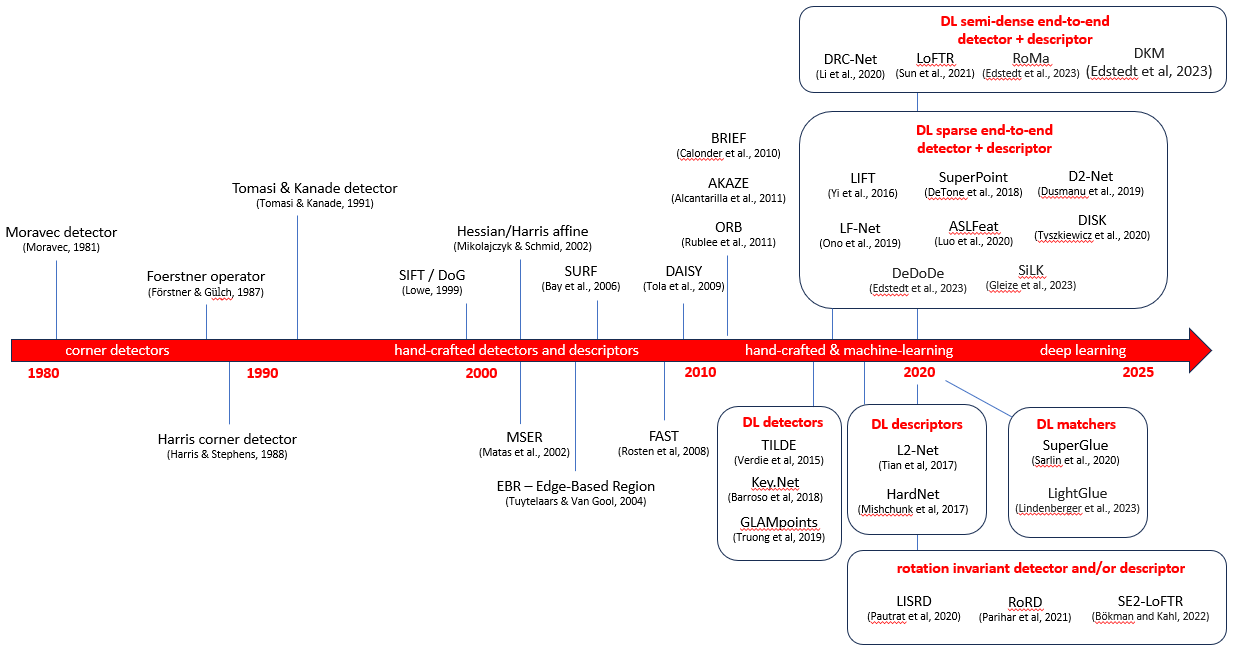
\includegraphics[width=1\textwidth]{local_feats_history}
%     \caption{Timeline development of detectors, descriptors and matchers from preliminary works, hand-crafted, machine-learning, and deep-learning local features. (Cit.)}
%     \label{fig:5:feats_history}
% \end{figure}

\section{Limitation of Deep Learning local features}\label{sec:5:limitation_dl_feats}

As discussed in \secref{sec:4:localfeatures}, in the past few years, a large number of trainable algorithms for robust local feature extraction and matching have been developed \citep{Yao_2021, remondino2022_at_with_dl}.
DL techniques, and particularly attention-based architectures~\citep{vaswani2023attention}, have emerged as a powerful technique for extracting and matching features in difficult conditions, such as wide baselines and significant radiometric differences~\citep{jin_image_2021, Yao_2021}.

Although DL local features offer several advantages, their limited rotational invariance remains a constraint, particularly when analyzing images with diverse orientations. 
While some initial studies highlighted this issue, many subsequent approaches have not prioritized solutions. 
This may stem from the common use of datasets with minimal rotational variability (e.g., upright images) within the computer vision community, which are common in aerial and UAV photogrammetric datasets \cite{Bkman2022_se2loftr}. 
Recently, some end-to-end approaches like LIFT \citep{yi2016lift} and LFNet \citep{ono2018lfnet}, and semi-dense methods like RoRD \citep{parihar2022rord} and SE2-LoFTR \citep{Bkman2022_se2loftr}, demonstrate progress in achieving rotational invariance. 
Recent works with Steerable CNNs \citep{cohen2016steerable}, which are examples of group equivariant neural networks that allow for \textit{steering} the descriptors to make them invariant by the rotation, further address this limitation \cite{Bkman2022_se2loftr, bokman2023steerers}.
Nevertheless, the number of approaches specifically addressing this problem is minimal compared to the overall interest in DL-based feature-matching algorithms.
On the other hand, the most common approach to address large rotation is still to compensate by iteratively rotating images during matching, but this becomes computationally intensive for large datasets.

Another limitation of DL approaches is their computational expense, which makes them unsuitable for deployment on full-resolution images, which are crucial for leveraging the available radiometric information in high-accuracy photogrammetric applications.
In addition, it's worth noting that training itself often occurs on low-resolution images, a concern highlighted in \cite{Wu2024_evaluation_dlstereo}, whose impact remains uncertain.
Training could have been generalized enough not to require additional training on high-resolution images. 

While the potential of these approaches under extreme lighting conditions and radiometric variations is increasingly evident \textcolor{red}{[Ref]}, some preliminary experiences suggest that these approaches may lack locally accurate identification \textcolor{red}{[Ref]}. 
Indeed, despite the existence of DL approaches for several years, their utilization in photogrammetric applications remains relatively limited. 
\textcolor{red}{[Include relevant papers: satellite image analysis, glacier monitoring, and applications aimed at enhancing augmented reality (AR) and virtual reality (VR) experiences, registering laser scanner point clouds, Precision Agriculture Agriculture (Gao et al., 2024)]}.

\begin{figure}[ht]
    \centering
    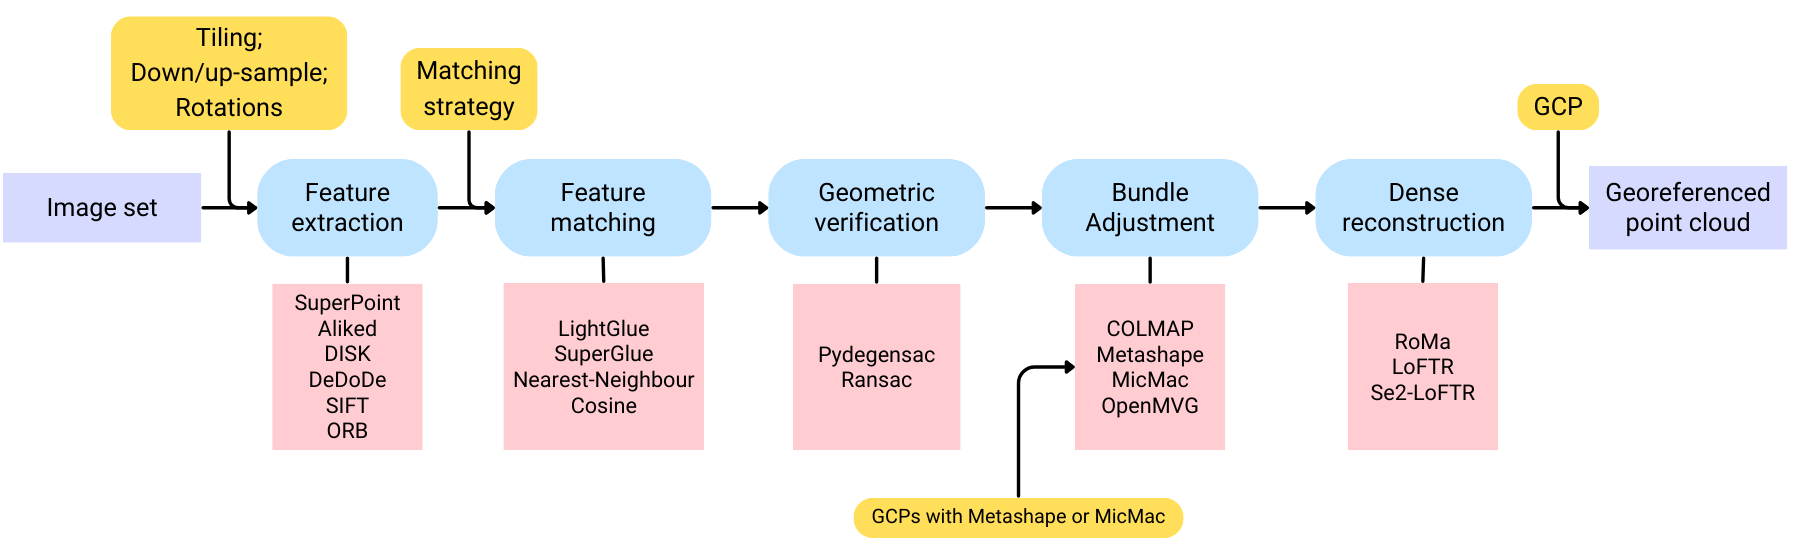
\includegraphics[width=1\textwidth]{dim_workflow_simple}
    \caption{Scheme of the DIM workflow.}
    \label{fig:5:dim_workflow}
\end{figure}

\section{Deep-Image-Matching}

% Given a set of unordered images, Deep-Image-Matching can perform the matching operations and return the corresponding points between images. It is developed in Python and publicly available on GitHub (\url{https://github.com/3DOM-FBK/deep-image-matching}), it supports both CLI and GUI as well as a wide range of local features and matching algorithms, spanning from the traditional ones to recent state-of-the-art learning approaches. Available local features include ORB, SIFT, SuperPoint (DeTone et al., 2020), ALIKE (Zhao et al., 2022), ALIKED (Zhao et al., 2023), DISK (Tyszkiewicz et al., 2020), Key.Net (Barroso-Laguna et al., 2019) + HardNet8 (Pultar, 2020), DeDoDe (Edstedt et al., 2023b). SuperGlue (Sarlin et al., 2020), LightGlue (Lindenberger et al., 2023), LoFTR (Sun et al., 2021), SE2-LoFTR (Bökman and Kahl, 2022), and RoMA (Edstedt et al., 2023a) are implemented as matchers. Additionally, KORNIA python library (Riba et al., 2020) can be used for nearest neighbour matching.
% Image pairs to be matched can be chosen by the user (custom pair option), or they can be automatically selected by other strategies, including all possible pairs (brute force), sequential matching (sequential), or image retrieval using global descriptors (retrieval). Image pairs can also be chosen by running a brute force on low-resolution images to limit computational time (option matching lowres).
% For high resolution images (i.e., images with the longest edge larger than 5000 px), feature extraction and matching are carried out by tiling the images on a regular grid to fit into GPU memory, while the selection of the tiles to be matched is guided by a first matching on low-resolution images. Features matched on each image pair are verified by using PyDegensac (Mishkin et al., 2015) to reject outliers. Geometrically verified tie points are then stored in a SQLite3 database to be imported in COLMAP, or in the openMVG format, ready for the bundle adjustment in the respective software. To import the solution in other photogrammetric software (e.g. Metashape), image orientation is performed with pycolmap library, and 3D tie points are exported in the Bundler format (Snavely et al., 2006).

Deep-Image-Matching\footnote{\url{https://github.com/3DOM-FBK/deep-image-matching}} (DIM) is a flexible, open-source Python library designed for robust multi-view image matching, leveraging both hand-crafted and DL matching techniques.  
Given a set of unordered images, DIM can perform the matching operations and return the corresponding points between images, providing the essential foundation for bundle adjustment and accurate photogrammetric reconstruction.

DIM's primary goal is to provide a user-friendly interface to a wide selection of state-of-the-art computer vision algorithms for matching and tracking corresponding points across unordered images.
Additionally, DIM aims to overcome the main limitations of DL-based matching approaches that pose challenges for their practical usage in photogrammetry and remote sensing. 
These limitations include sensitivity to rotation changes, computational bottlenecks with high-resolution images (e.g., larger than 3000 px on the longest edge), difficulties in achieving sub-pixel accuracy, inefficient image pair selection for large datasets, and compatibility issues with existing SfM software packages.  

DIM employs a modular workflow designed for effective multi-view matching \figref{fig:5:dim_workflow}.
DIM itself does not perform the bundle adjustment and scene reconstruction, but it is designed to ensure seamless integration with various popular SfM software packages within the remote sensing and computer vision communities. 
These include COLMAP \citep{schoenberger2016sfm}, OpenMVG \citep{moulon2016openmvg}, MicMac \citep{rupnik2017micmac}, Agisoft Metashape\footnote{\url{https://www.agisoft.com/}}, 
and any other software package that supports the import from a Bundler solution format \citep{Li_Snavely_2018_MegaDepth}.
Additionally, DIM can be easily integrated into a multi-camera multi-epoch pipeline, e.g., by exploiting the multi-temporal functionalities of ICEpy4D (see \chref{ch:4}).

The process begins with a pre-processing stage where users select from different matching strategies (brute-force, low-resolution guided, sequential, image retrieval, or custom) to intelligently select the pair of images for optimized matching. 
Additionally, DIM provides a module for addressing the challenge of rotated images within datasets (e.g., in the case of aerial or UAV surveys) by automatically identifying the ideal rotation angle between image pairs, significantly boosting matching accuracy. Users can opt to match images at their original resolution or employ down-sampling or up-sampling techniques managed by a quality parameter.
To handle high-resolution imagery, DIM offers the added capability of image tiling, ensuring efficient processing without compromising detail. 

For the actual matching, DIM supports various combinations of local feature and matching algorithms, named \textit{pipelines}, optimized for diverse problem domains. This allows users to tailor the workflow to their specific needs. 
Each pipeline consists of two main components: (i) an \textit{extraction} step that is responsible for extracting local features from all images in the dataset; and (ii) a \textit{matching} step that matches the extracted local features across the image pairs selected by the chosen matching strategy.  

DIM supports a wide range of local features and matching algorithms, spanning from the traditional ones to recent state-of-the-art learning approaches. 
Available local features include ORB \citep{Rublee2011}, SIFT \citep{Lowe2004}, SuperPoint \citep{DeTone_2018}, 
ALIKE \citep{zhao2022alike}, ALIKED \citep{zhao2023aliked}, DISK \citep{tyszkiewicz2020disk},
Key.Net \citep{barrosolaguna2019keynet} + HardNet \citep{pultar2020improving}, DeDoDe \citep{edstedt2024dedode}.
DIM implements SuperGlue \citep{sarlin2020superglue}, LightGlue \citep{lindenberger2023lightglue}, and traditional nearest-neighbor algorithms based on the KORNIA library \citep{riba2019kornia} as local features matchers. 
Additionally, the detector-free matchers algorithms LoFTR \citep{sun2021_loftr}, SE2-LoFTR \citep{Bkman2022_se2loftr}, and RoMA \citep{edstedt2023roma} are included in DIM and allows for a semi-dense scene reconstruction.

\subsection{Matching strategies}\label{sec:5:matching_stategies}

\begin{figure}[ht]
  \centering
  \subcaptionbox{Unordered set\label{fig:5:matching_strategy:unordered}}{
    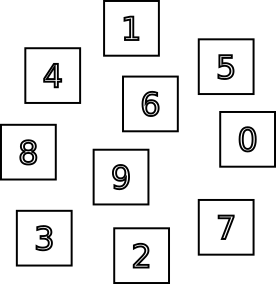
\includegraphics[height=3.5cm]{match_strat_unordered}
  } \qquad
  \subcaptionbox{Bruteforce\label{fig:5:matching_strategy:bruteforce}}{
    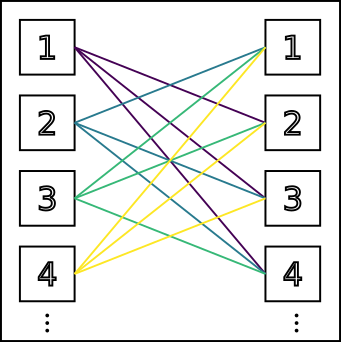
\includegraphics[height=4cm]{match_strat_bruteforce}
  }\\ \vspace{2mm}
  \subcaptionbox{Sequential (overlap=2)\label{fig:5:matching_strategy:sequential}}{
    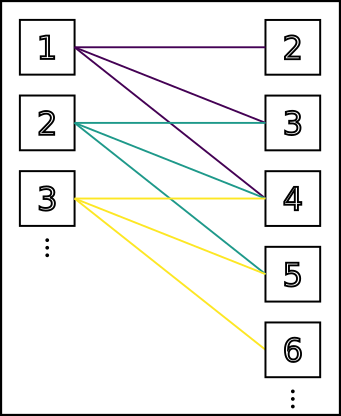
\includegraphics[height=5cm]{match_strat_sequential}
  }\qquad
  \subcaptionbox{Low-res preselection\label{fig:5:matching_strategy:lowres}}{
    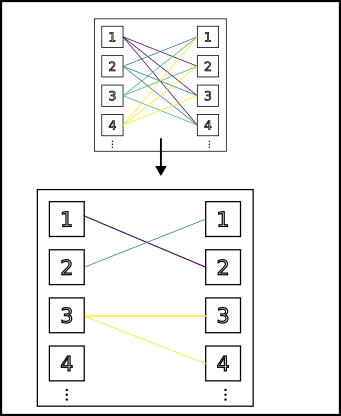
\includegraphics[height=5cm]{match_strat_lowres}
  }  
  \caption{Scheme of the main different matching strategies implemented in DIM given an unorered image set (a). (b) Bruteforce strategy (i.e., \textit{all-to-all)}; (c) Sequential strategy with overlap equal to 2 (i.e., match all images with next 3 images, note that the overlap parameter is zero-based); (d) Low-resolution guided matching strategy (i.e., perform a fast bruteforce on low-resolution images and match only good candidates at high resolution).}
  \label{fig:5:matching_strategy}
\end{figure}

The matching strategy defines how the pairs of images to be matched are selected to optimize the matching process. The choice of matching strategy plays a crucial role in optimizing image matching, especially with large datasets.  

DIM offers a versatile range of strategies to address diverse use cases. 
The \texttt{brute-force} approach provides the most comprehensive exploration by attempting to match every image with every other (\figref{fig:5:matching_strategy:bruteforce}). 
This method is computationally intensive but can be valuable for small datasets or complex scenarios where other strategies may yield insufficient matches. 
The image pairs are obtained by computing combinations of n elements in 2 places, where n is the number of images in the dataset. 
Therefore, the computation complexity by $ p = C(n,2) = \frac{n*\left(n-1\right)}{2}$, where $p$ is the number of pairs.

For image sequences acquired in order by a moving camera, (e.g., Visual Odometry or SLAM), the \texttt{sequential} strategy offers optimized efficiency by matching each image with a defined number of subsequent images. 
The overlap parameter defines the number of consecutive images to match sequentially (\figref{fig:5:matching_strategy:sequential}).
The computational complexity is given by $p = \left(n-O\right) * O $, where $O$ is the overlap parameter.

The \texttt{matching\char`_lowres} enhances computational efficiency by initially analyzing downsampled images to pre-filter pairs based on valid matches detected at lower resolution and considered as inliers after a geometric verification (\figref{fig:5:matching_strategy:lowres}). 
By default, the minimum number of valid matches is 20 but it can be tuned by the user. 

The \texttt{retrieval} strategy allows to use of global features to determine the pairs of images that are likely to see the same scene \citep{Yang2013_imageretrieval}. 
Global features encode the full images into a neural network and therefore they are widely used to tackle visual place recognition problems \citep{napoletano2017visual}. 
DIM makes use of hloc \citep{Sarlin_2019_hloc} for extracting and matching global features and it supports NetVLAD \citep{arandjelovic2016netvlad},  openIBL \citep{ge2020selfsupervising}, and CoSpace \citep{Hong_2019} global features.  

Finally, the \texttt{custom\char`_pairs} option grants users precise control over the matching process, allowing the specification of exact image pairs via a text file. 
This enables tailored workflows for specific research objectives. 

\subsection{Image resolution and tiling}\label{sec:5:tiling}

DIM provides extensive control over image resolution before feature extraction and matching, providing flexibility for different user needs and hardware constraints. 
This functionality is particularly important when using DL-based local feature extractors and matchers that rely on GPU parallelization for best performance. 
They face limitations when processing large images on consumer-grade GPUs, which typically have limited memory resources. 
The image size threshold varies depending on the available GPU memory and the specific algorithms used (detector-free matchers tend to be particularly memory-intensive). 
As a general guideline, images with a long edge of up to 3000 pixels can often be processed on a 12GB GPU using a combination such as SuperPoint and LightGlue. 

To address this challenge, DIM offers several resolution management strategies: images can be downsampled by a factor of 2, 4, or 8 (medium, low, or lowest quality settings in DIM) using OpenCV's pixel-area relation (bilinear interpolation). 
This approach may be appropriate when computational efficiency is a priority. Alternatively, for DL features that operate with pixel-level accuracy (e.g., SuperPoint), upsampling by a factor of 2 (DIM's highest quality setting) using bicubic interpolation can improve subpixel detection capabilities.  

To preserve high-resolution detail in large images, DIM supports breaking them into smaller, regular tiles.
This is critical when using end-to-end detector-free matchers (e.g., LOFTR, RoMa), as their combined extraction and matching steps are particularly memory intensive. 
DIM's tiling allows the user to specify tile dimensions or the number of tiles per row/column.
An overlap between neighboring tiles can be specified to avoid having no features extracted along the tile boundaries. 
The software automatically handles zero padding to maintain consistent tile sizes throughout. 

When using image tiling, DIM handles local feature extraction separately, processing each tile sequentially. 
However, tile-based feature matching offers several strategies: \texttt{exhaustive}, \texttt{preselection}, and \texttt{grid} mode.
In \texttt{exhaustive} mode, features from each tile of the first image are matched against features extracted from all tiles of the second image. 
This mirrors the brute-force approach to image pair selection (see \secref{sec:5:matching_stategies}) and ensures comprehensive exploration of potential matches, but can be computationally intensive. 
The \texttt{preselection} mode prioritizes efficiency and is the default approach. 
An initial low-resolution matching step identifies tile pairs likely to contain corresponding features, reducing computational cost by focusing subsequent matching efforts. 
\texttt{Grid} mode assumes a high degree of similarity between the two images. 
It matches features from each tile in the first image to features from the corresponding tile (i.e., the tile that shares the same boundaries in image coordinates) in the second image. 
This approach is well suited for scenarios such as VSLAM, where images are captured sequentially by a moving camera and represent similar scenes. 

\begin{figure}[hb!]
  \centering
  \subcaptionbox{\label{fig:5:rotations:1}}{
    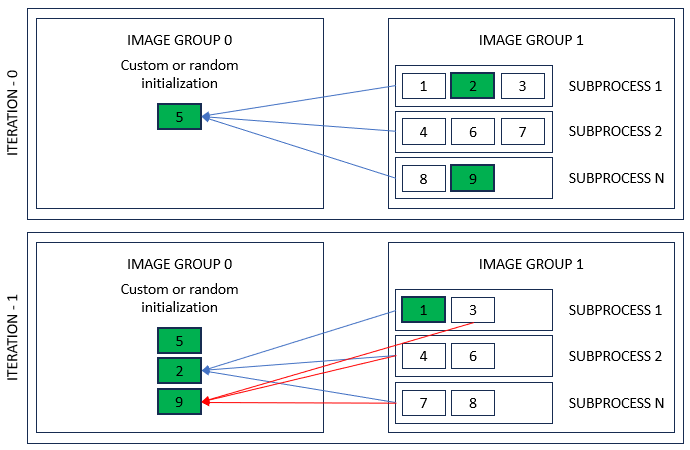
\includegraphics[width=.8\textwidth]{dim_rotations_1.png}
  } \\
  \subcaptionbox{\label{fig:5:rotations:2}}{
    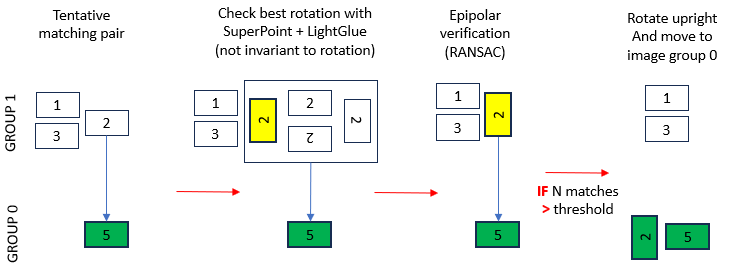
\includegraphics[width=1\textwidth]{dim_rotations_2.png}
  }
  \caption{Scheme of the DIM's cluster-based approach to estimate the best rotation of the images before performing the image matching.}
  \label{fig:5:dim_rotations}
\end{figure}

\subsection{Image rotations}

DL-based local features often struggle with extreme image rotations because they are trained on datasets with largely consistent orientations. 
DIM addresses this challenge with two management approaches ensuring images are properly rotated according to a \textit{principal direction} before feature extraction and matching.
Features are extracted and matched from the rotated images, and only after matching are keypoints mapped back to their positions in the original image.

If the images' orientation relative to a principal direction is known (e.g., from on-board positioning systems), DIM accepts a text file specifying these rotations and rotates the images accordingly.
Alternatively, in the absence of prior rotation knowledge, a \textit{2-cluster approach} relative to a reference image (either random or user-selected) can be used to determine the principal direction (\figref{fig:5:dim_rotations}).
This iterative method starts with a single reference image in the first cluster (group 0) and all remaining images in the second cluster (group 1). 
Each image $I_i$ in Group 1 is iteratively matched against a reference image $I_r$ in Group 0, testing rotations of [90, 180, 270] degrees. 
The rotation with the highest number of geometrically verified matches is selected. 
If the number of matches exceeds a predefined threshold, $I_i$ is moved to group 0, expanding that cluster and reducing group 1. 
This procedure is parallelizable, with group 1 images divided into subgroups for independent matching against group 0 images on independent processes.
This significantly speeds up the computational time compared to a brute-force approach. 

\subsection{Matching pipelines}

DIM offers flexibility by supporting diverse pipelines for image matching. 
A \texttt{pipeline} consists of a local feature extractor and its corresponding matching algorithm. 
As compatibility constraints exist between feature extractors and matching algorithms within DL-based methods, DIM currently supports the following pipelines:
\begin{itemize}
    \item SuperPoint+LightGlue
    \item SuperPoint+SuperGlue
    \item DISK+LightGlue
    \item Aliked+LightGlue
    \item ORB+nearest neighbor matching
    \item SIFT+nearest neighbor matching
    \item KeyNetAffNetHardNet+nearest neighbor matching
    \item DeDoDe+nearest neighbor matching
    \item LOFTR (detector-free matcher)
    \item RoMa (detector-free matcher)
\end{itemize}

DIM streamlines the process with a unified interface, allowing users to run pipelines with minimal configuration when default settings are suitable. 
For customization of local feature extractor or matcher parameters, advanced users can provide configuration files to DIM's image-matching interface.

DIM efficiently stores extracted features and matches in local HDF5 (Hierarchical Data Format) databases, by using the h5py library\footnote{h5py library: \url{https://docs.h5py.org/en/stable/}}. 
Pipeline outputs are stored in two HDF5 files: \textit{features.h5} containing keypoints image coordinates, descriptors, and scores and \textit{matches.h5} containing the indices of matched features for each image pair. 
The features database organizes features by image, with datasets (i.e., a structure similar to a table in a relational database) representing extracted features on each image. 
The matches database contains datasets per image pair, storing an nx2 array (n = number of matches) where columns reference the corresponding feature indices within the feature database. 
This indexing enables the construction of tracks, which build tracks of features matched across multiple images. 
Additionally, this easy-to-use structured format enhances flexibility and maintainability.

The use of HDF5 facilitates the combination of pipelines and the merging of feature sets. 
This enables the strategic exploitation of different local feature strengths; for example, the same set of images can be processed both with SIFT to exploit its accuracy and reliability for standard baselines and with DL-based algorithms like SuperPoint+LightGlue due to its robustness for wide baselines and significant viewpoint changes.

After completing the matching pipelines, outlier correspondences must be rejected. 
DIM assumes non-calibrated cameras and employs Fundamental matrix estimation for this purpose, rejecting matches with large epipolar errors. 
DIM offers a robust selection of algorithms for Fundamental matrix estimation and geometric verification. 
Among these, PyDegensac \cite{Mishkin2015_pydegensac}, implementing LO-Ransac \cite{Chum2003_loransac} and DEGENSAC \cite{Chum2005_degensac}, provides the most robust solution.  Additionally, DIM supports all robust estimation algorithms implemented in OpenCV\footnote{OpenCV robust estimators: \url{https://docs.opencv.org/4.x/d9/d0c/group__calib3d.html}}, including traditional RANSAC, the least-median of squares algorithm (LMedS), and LO-Ransac (USAC\_DEFAULT).

% A sub-pixel refinement module allows for improvements in the matching precision, especially in the case of DL-based features that work only at the pixel level. 
% Different robust geometric verification techniques can be employed to verify the correspondances and to reject inaccurate or unreliable matches. 

% \subsection{Sub-pixel refinement and geometric verification}

% As many DL-based descriptors, including SuperPoint, work at the pixel level, DIM implements a sub-pixel routine after the matching to improve the accuracy of the image coordinates of the tie points. 
% To this end, DIM uses cross-correlation to refine the location of the matched keypoints.
% For each image pair that contains correspondences, DIM opens a series of small templates around each feature and tries to find the best location 
% Currently, DIM supports normalized cross-correlation and orientation correlation \cite{fitch2002_OC}, which is more robust against illumination changes \cite{Heid2012_evaluation_xcorr, Ioli2023_icepy4d}, as correlation functions to find the best location of the template in the second image.
% To achieve sub-pixel accuracy, the correlation matrix is upsampled by a factor of 10 by interpolating it with a bicubic function, and the correlation peak is found as the maximum of the interpolated correlation function \cite{Debella_Gilo2011}.

% As this approach requires a rather strong radiometric similarity of the keypoints' neighboorhod in the two images, it is suitable for normal baselines and not extreme viewing angles. 
% In these case, in fact, strong affinity-like distortions and occlusions may hinder the possibility to refine the tie point position based only on the radiometric similarity.
% Additionally, this approach may struggle in textureless cases or with strong scale variations. 

\section{Case studies}\label{sec:5:methods}

This section presents several case studies on challenging multi-view datasets, showcasing DIM's versatility in diverse remote sensing scenarios.
While these studies may not directly focus on the Belvedere Glacier, they address common complexities encountered in the remote sensing field.  
Furthermore, two case studies specific to the Belvedere Glacier demonstrate how DIM, integrated with ICEpy4D (see \secref{sec:4:stereoworkflow}), can enable the creation of effective multi-view monitoring systems using low-cost cameras.

% Even though they are not all specifically related to the Belvedere Glacier, they tackle specific challenging scenarios that may be commonly encountered in remote sensing.
% Two case studies related to the Belvedere Glacier introduce to the possibility of applying DIM for achieving an actual multi-view monitoring system using low-cost cameras, by integrating DIM with ICEpy4D (see \secref{sec:4:stereoworkflow}, used for tackling the multi-temporal component of the monitoring system. 

% \subsection{Dense reconstruction with wide-camera baselines}

% As discussed in \chref{ch:4}, the wide baseline of the stereo cameras installed at the Belvedere Glacier posed strong challenges in tie point extraction using traditional hand-crafted local features. 

% \begin{figure}
%   \centering
%   \subcaptionbox{\label{fig:5:stereo_res:1}}{
%     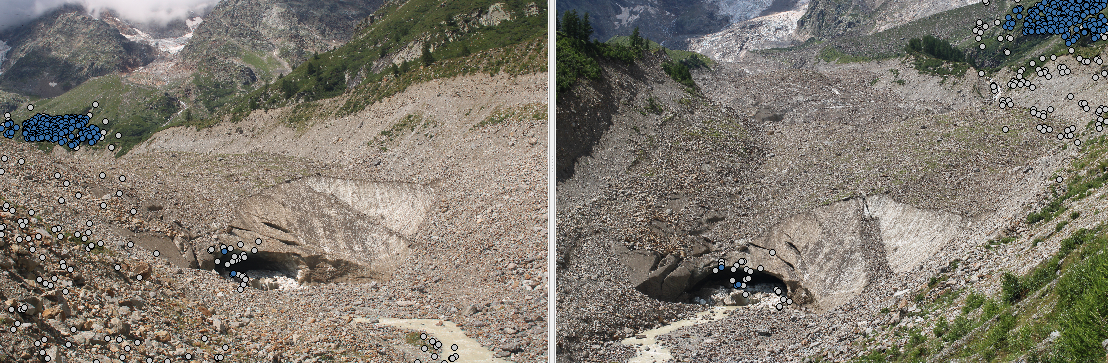
\includegraphics[width=12cm]{stereo_ms_matches}
%   }\\
%   \subcaptionbox{\label{fig:5:stereo_res:2}}{
%     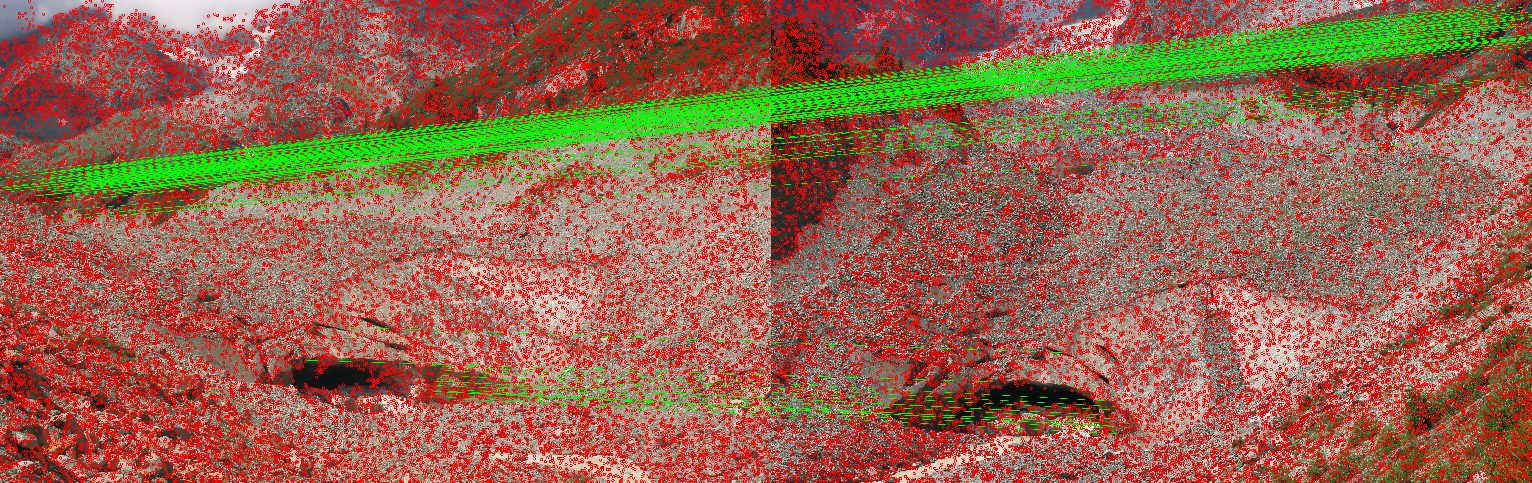
\includegraphics[width=12cm]{stereo_colmap_matches}
%   }\\
%   \subcaptionbox{\label{fig:5:stereo_res:3}}{
%     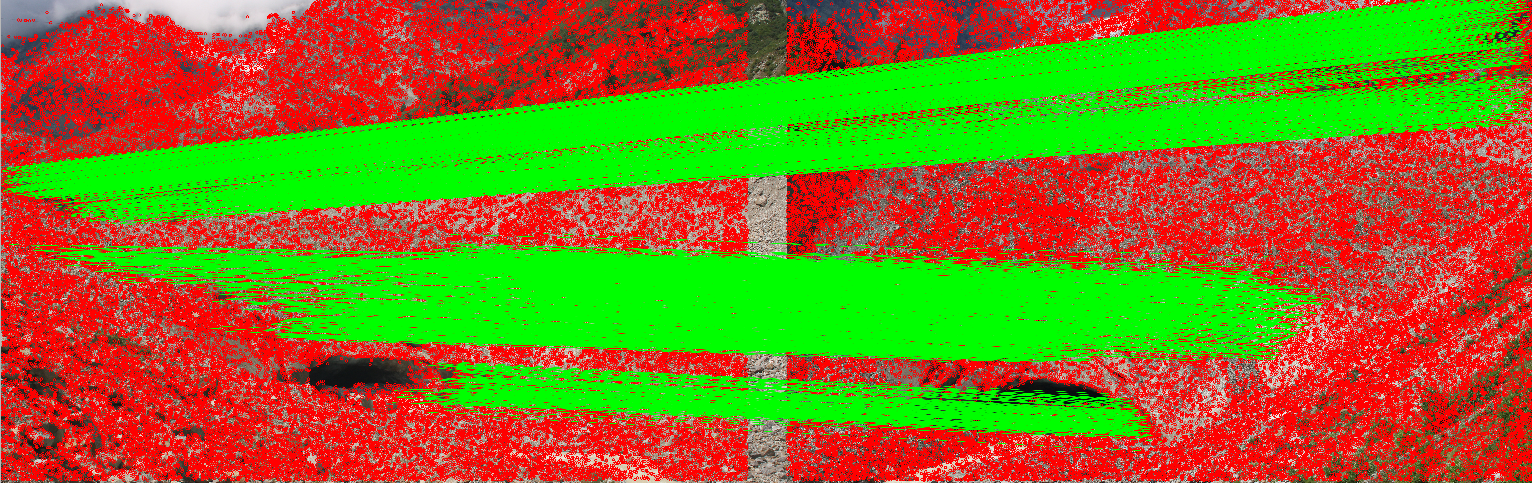
\includegraphics[width=12cm]{stereo_sp+lg_matches}
%   }
%   \caption{}
%   \label{fig:5:stereo_res_sparse}
% \end{figure}


% \begin{figure}
%   \centering
%   \subcaptionbox{\label{fig:5:stereo_dense:1}}{
%     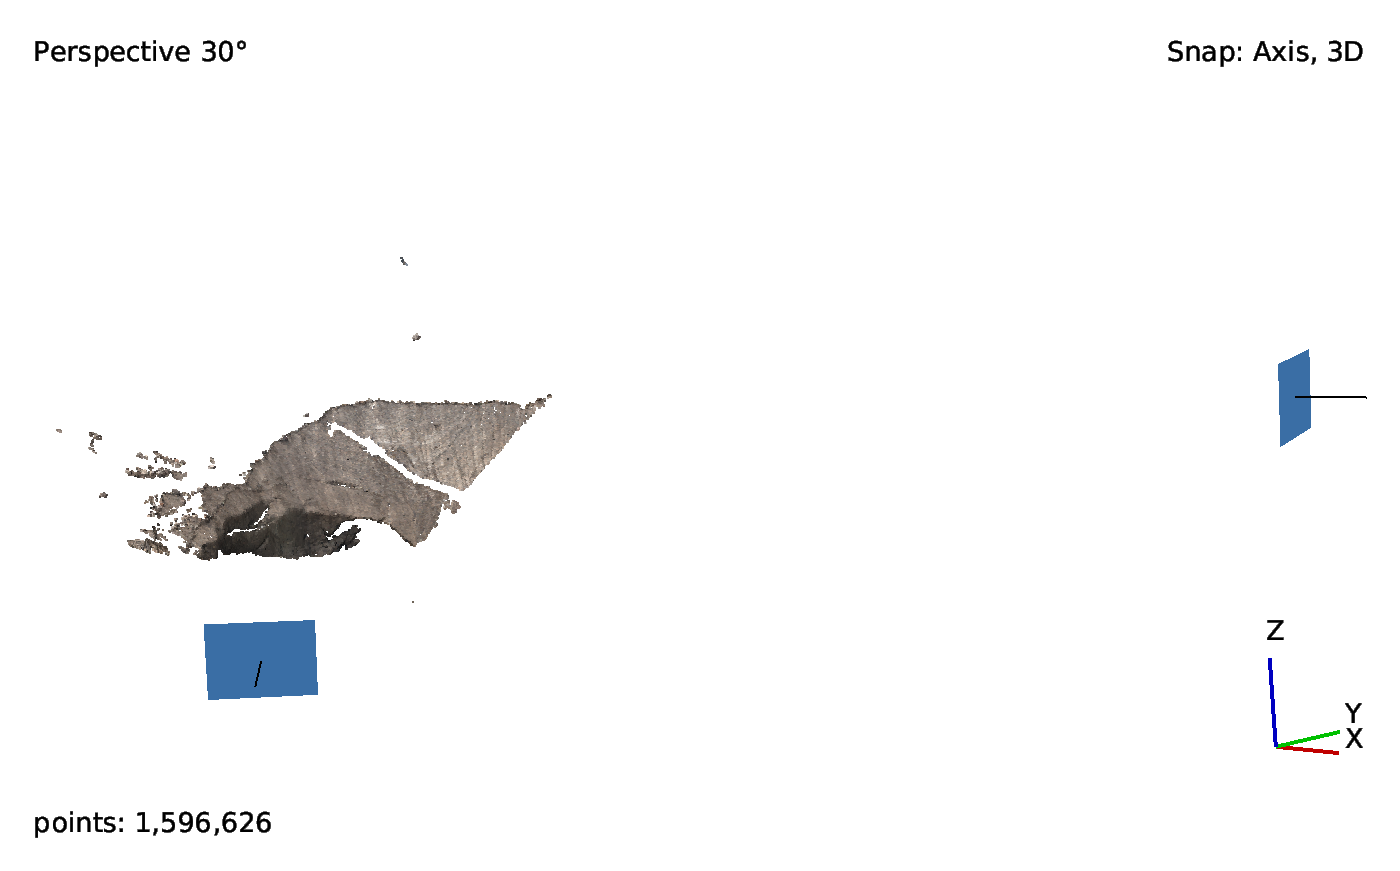
\includegraphics[width=12cm]{stereo_dense_from_splg}
%   }\\
%   \subcaptionbox{\label{fig:5:stereo_dense:2}}{
%     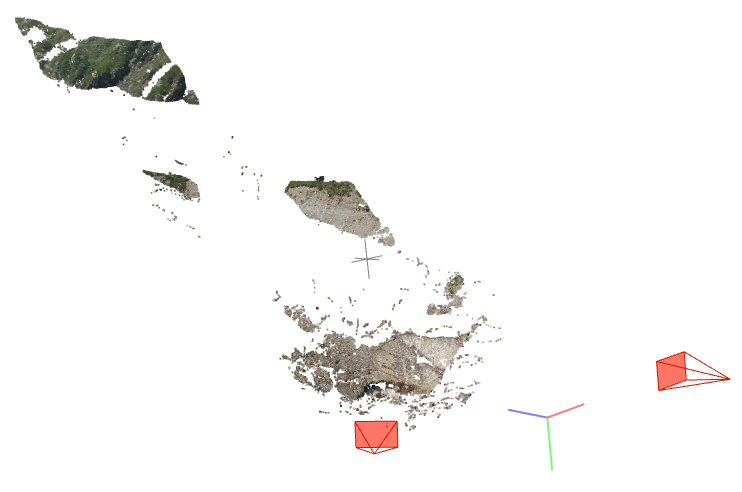
\includegraphics[width=12cm]{stereo_dense_roma}
%   }
%   \caption{}
%   \label{fig:5:stereo_dense}
% \end{figure}


\begin{figure}[ht]
  \centering
    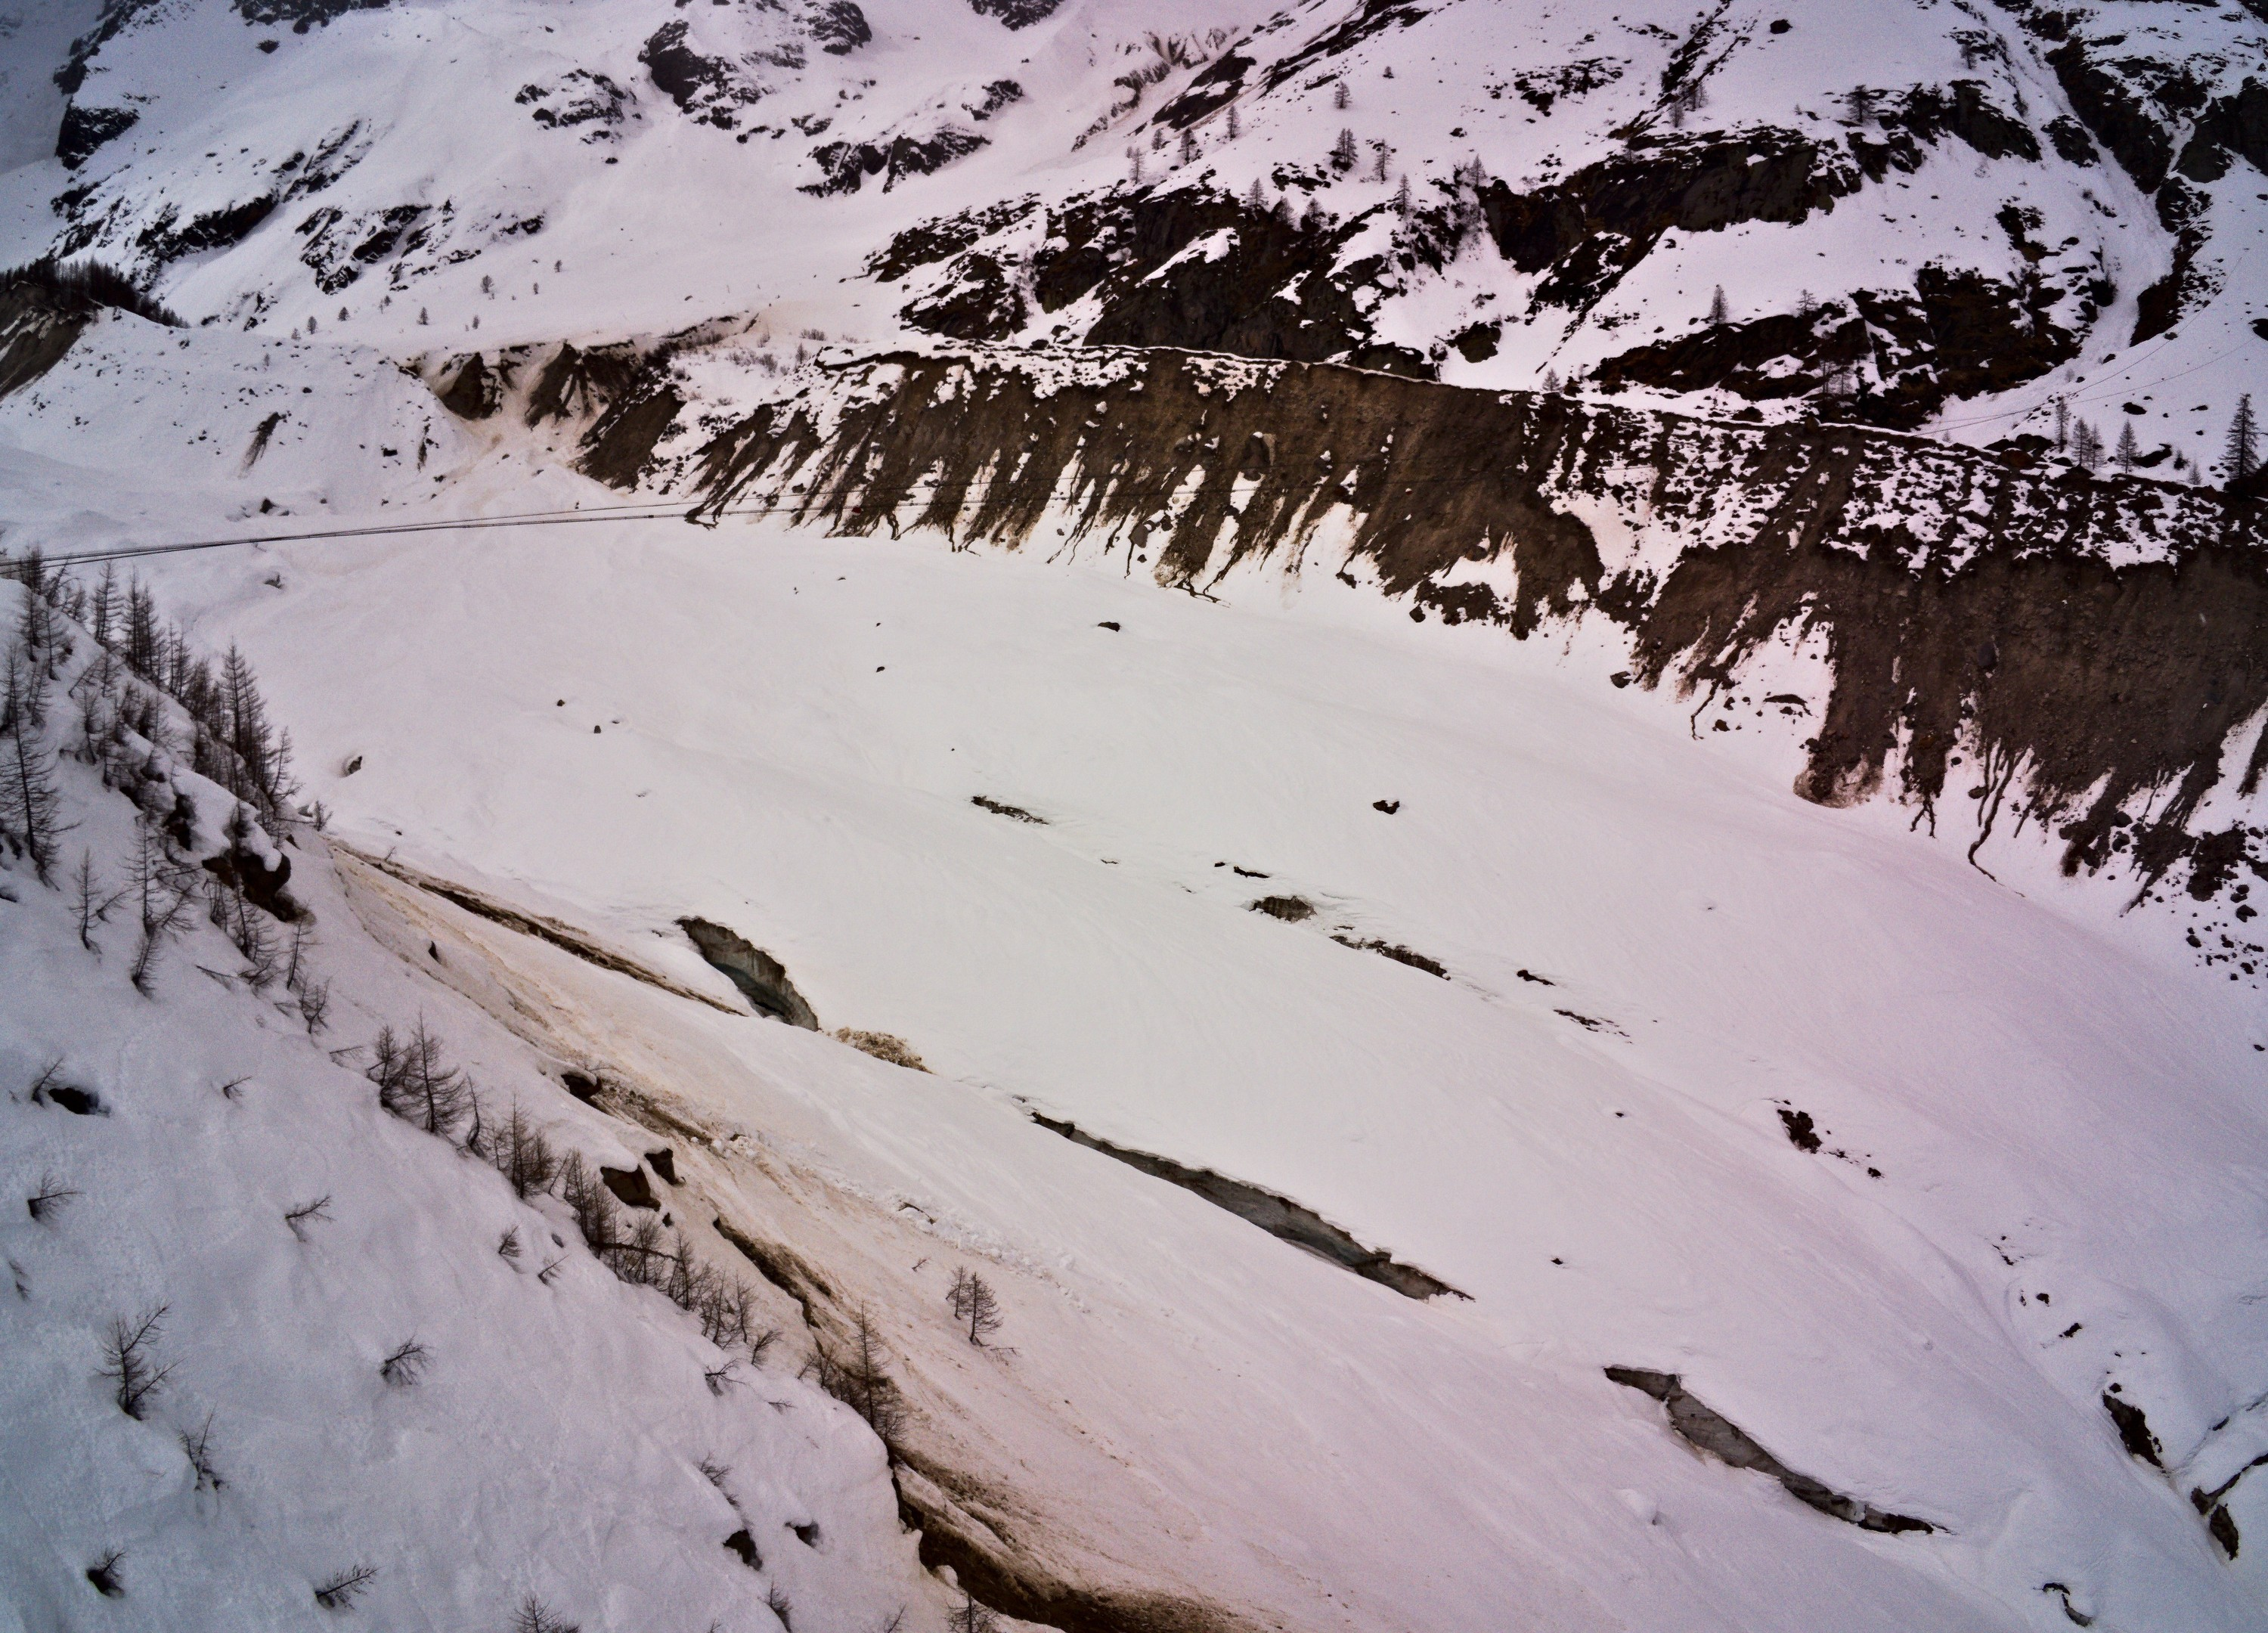
\includegraphics[height=3.5cm]{winter_img_1}
    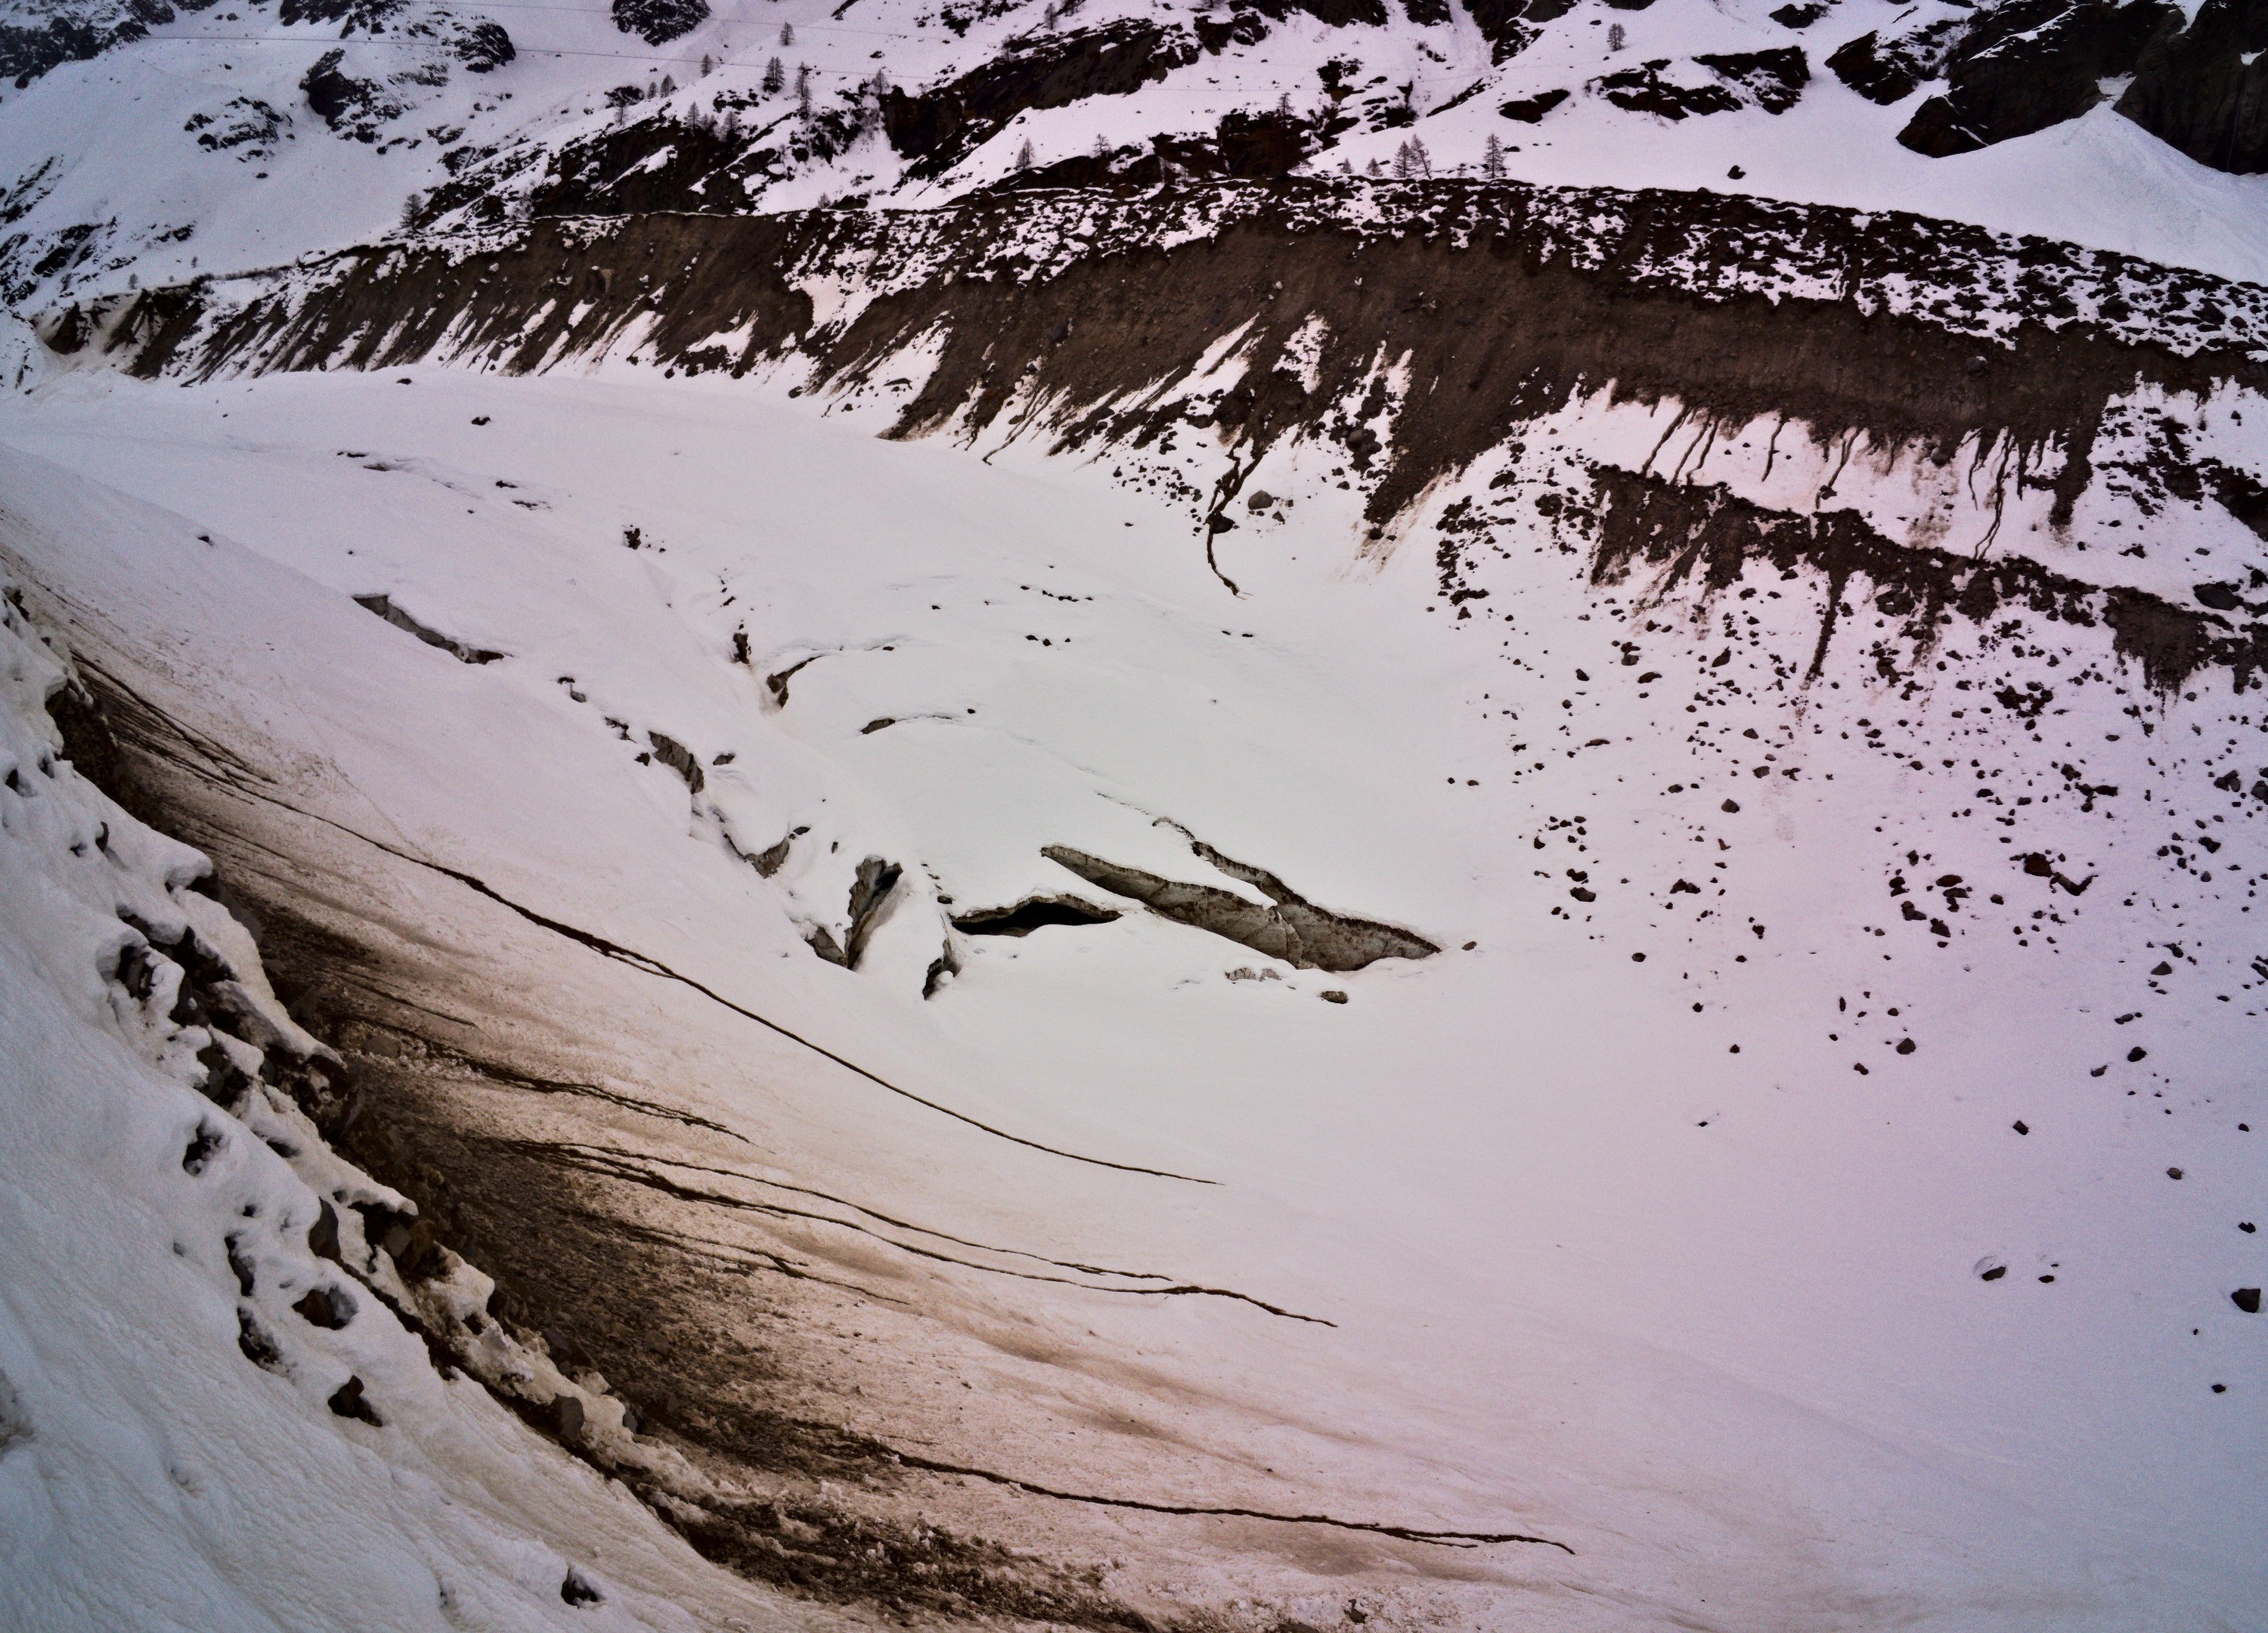
\includegraphics[height=3.5cm]{winter_img_2}
    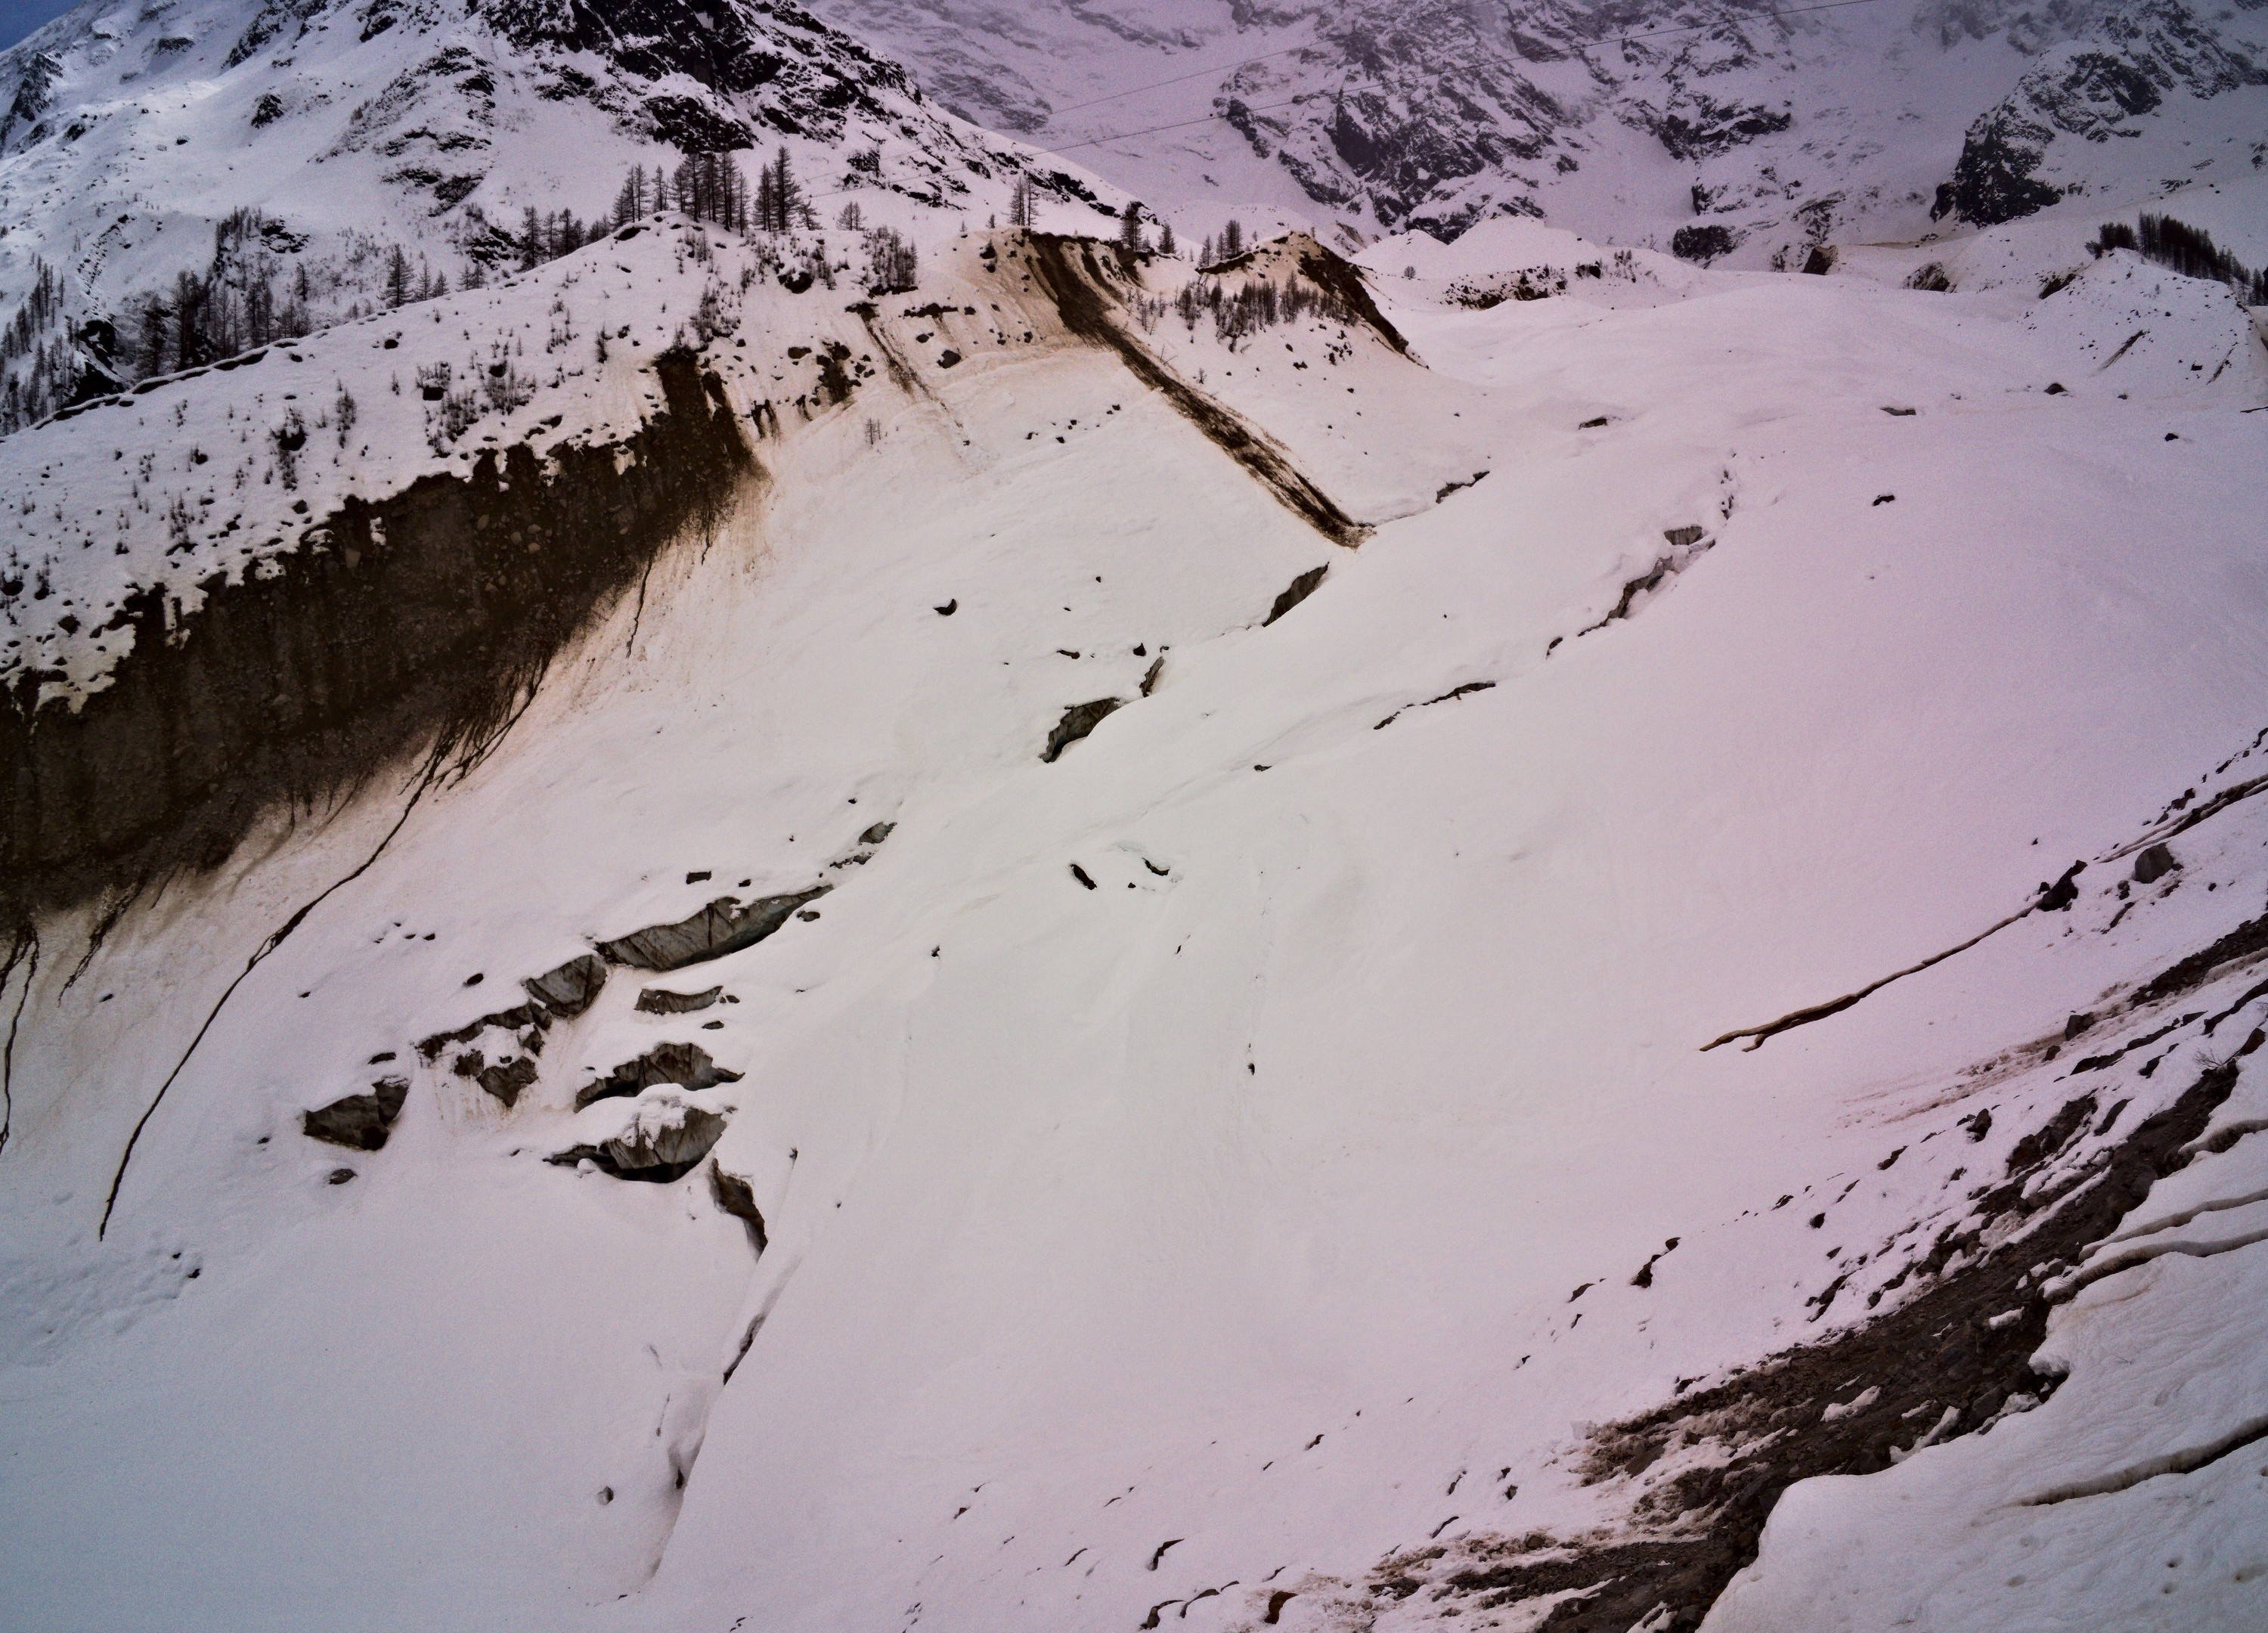
\includegraphics[height=3.5cm]{winter_img_5} \\ \vspace{1mm}
    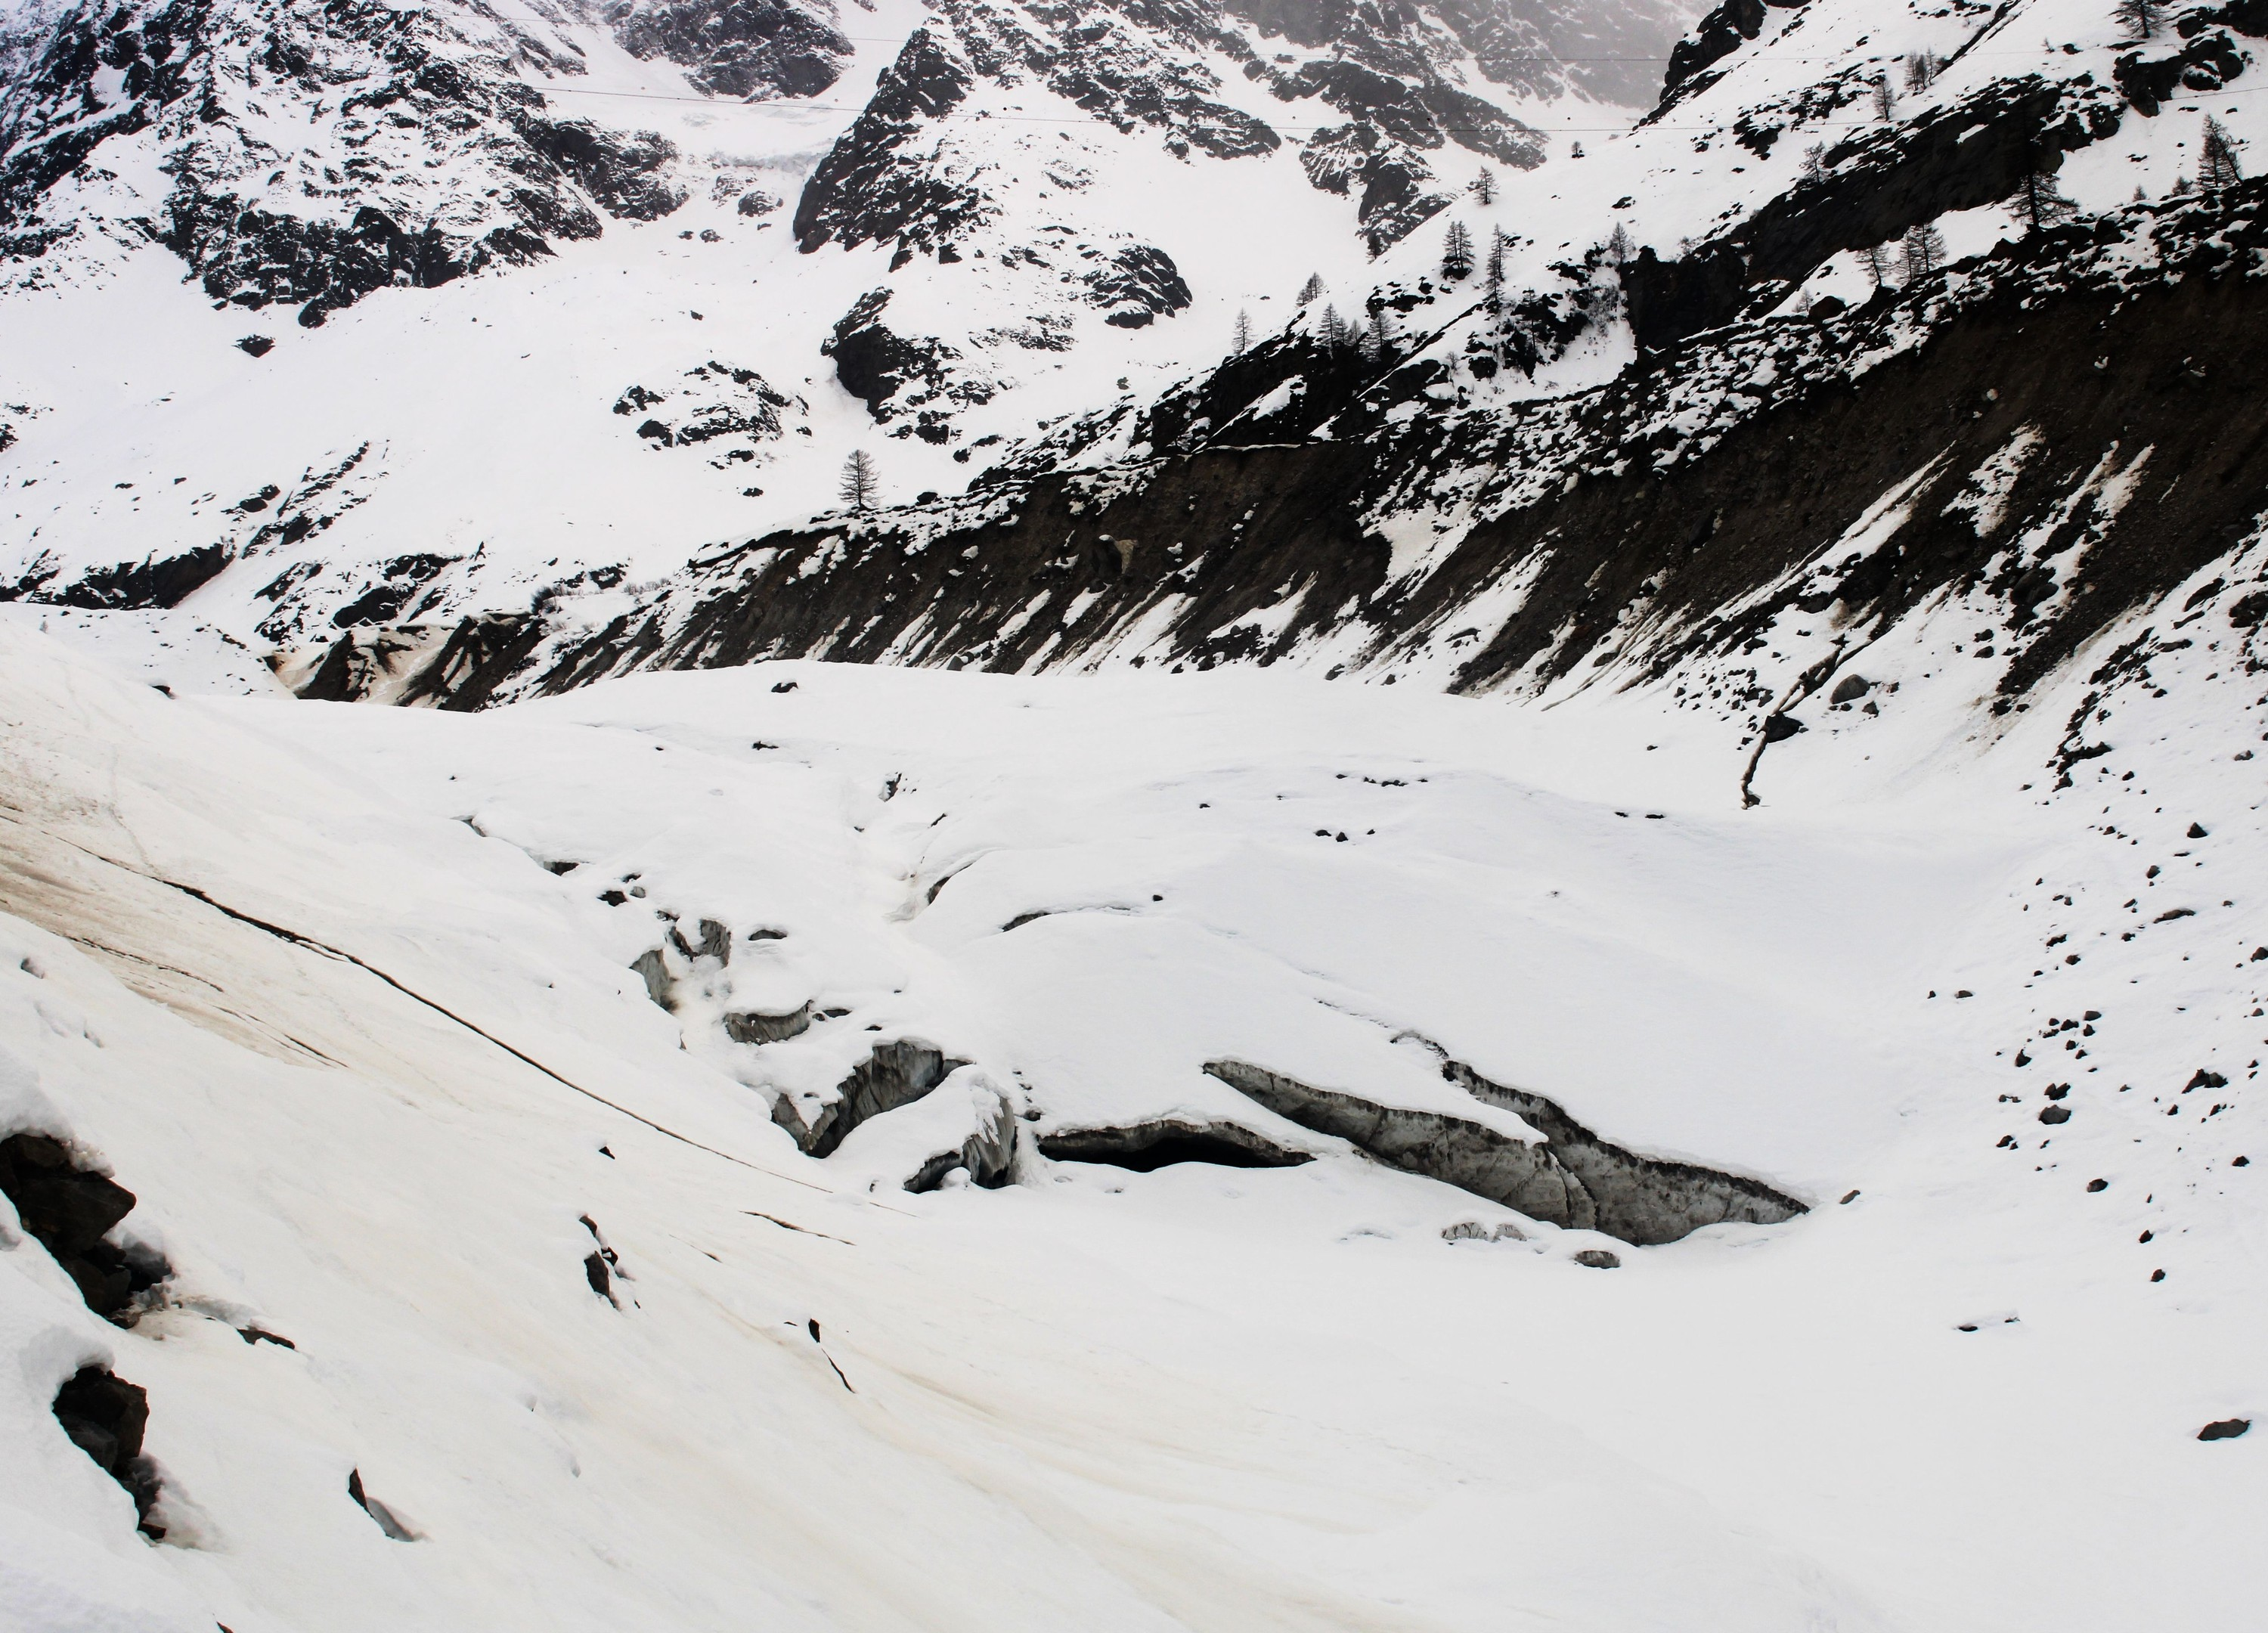
\includegraphics[height=3.5cm]{winter_img_3}
    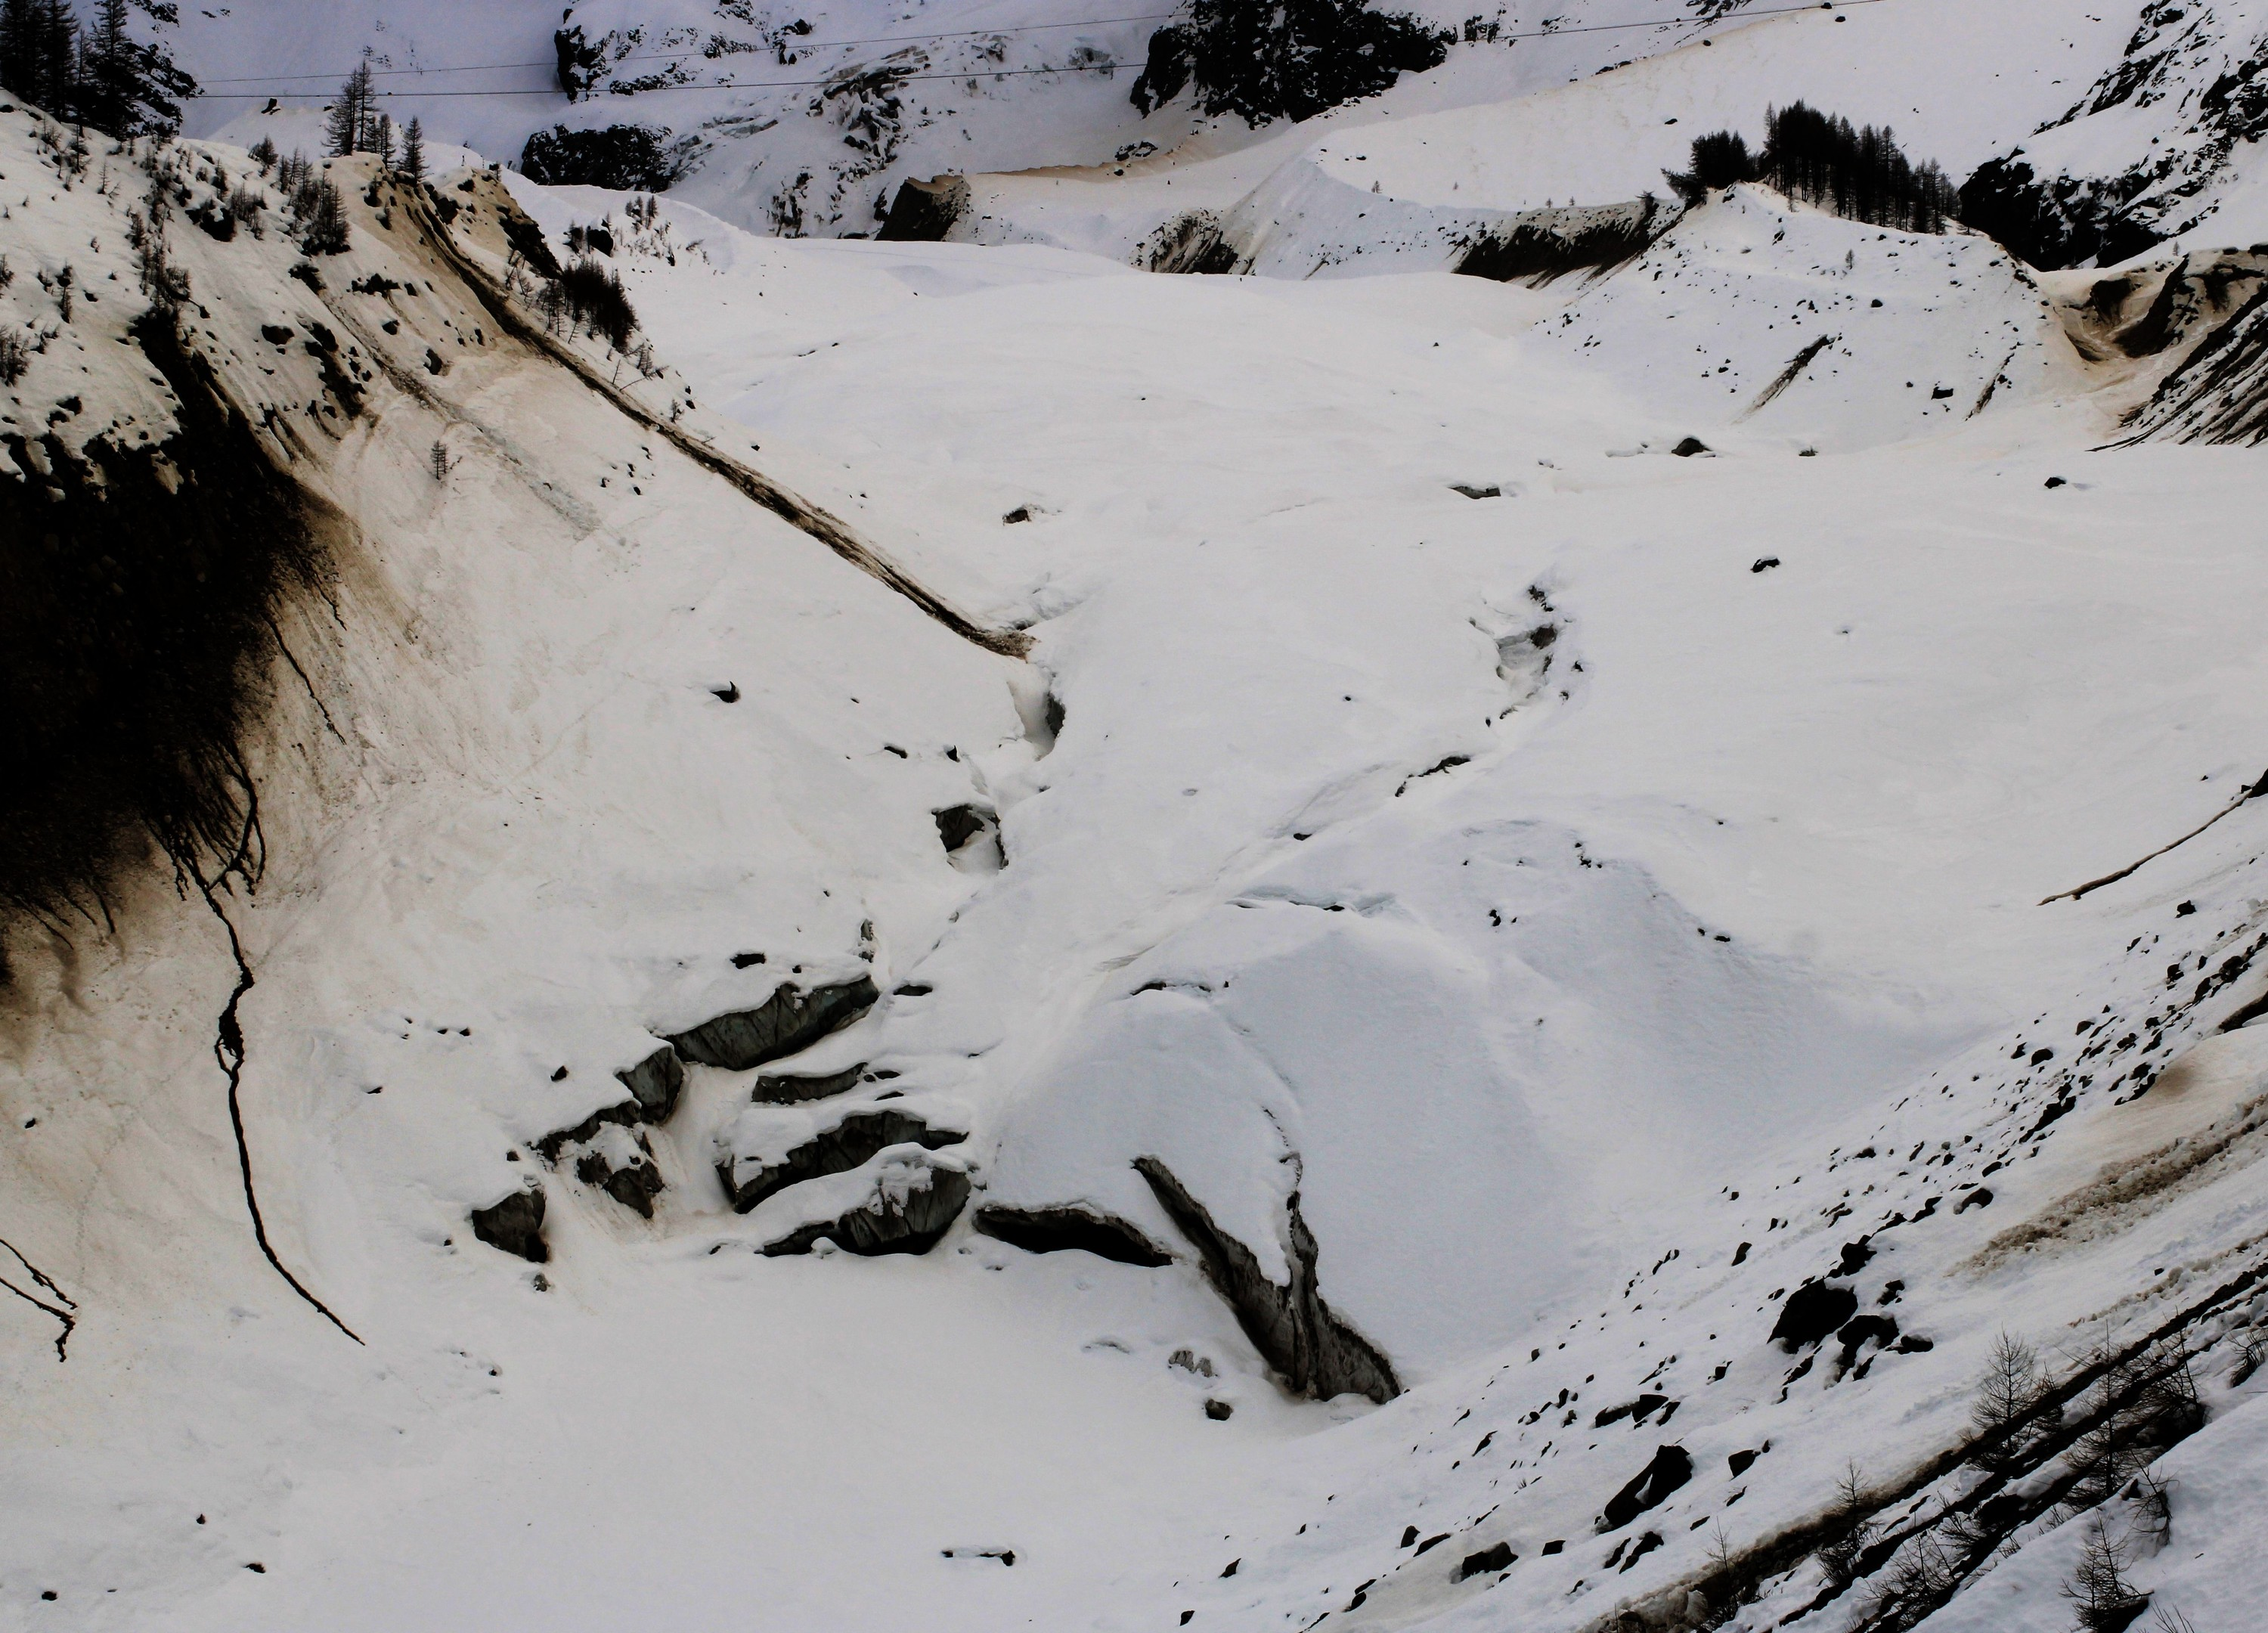
\includegraphics[height=3.5cm]{winter_img_4}
  \caption{Images of Dataset A - Winter. Images in the first row are taken by UAV, while those in the second row are acquired by the terrestrial cameras.}
  \label{fig:5:winter_images}
\end{figure}

\subsection{Low-textures scenes}

Hand-crafted descriptors like SIFT often struggle in low-texture environments, such as a snow-covered glacier.  
The lack of distinctive features significantly complicates finding corresponding points for image orientation. 
Since glaciers are commonly snow-covered for large parts of the year, addressing this challenge is essential for robust, long-term monitoring.
While the time series analysis discussed in \chref{ch:4}was limited to the May-November period, the planned expansion to a multi-camera system motivated a focused investigation into this scenario. 
To simulate a multi-view setup, we integrated the 24/03/2024 images captured by the existing two fixed cameras with three additional images acquired by a Parrot Anafi UAV (1/1.2.4" CMOS sensor with 4.8 mm focal length - 23 mm in 35mm format equivalent).
Dataset A - Winter - is composed of these three UAV images, acquired from positions near potential future camera locations along the glacier moraines and with convergent view angles, combined with the two terrestrial images (\figref{fig:5:winter_images}).

\begin{table}[ht]
    \centering
    \caption{Summary of the Winter dataset results obtained with DIM compared to those obtained with COLMAP (with RootSIFT features) and Agisoft Metashape with its proprietary feature extractor and matches.} 
    \label{tab:5:winter_statistics}
    
    \begin{tabular}{l p{3.5cm} p{2.2cm} p{2.2cm} p{2.2cm} p{2.2cm}}
    \toprule
    &Local features \newline and matcher & Oriented/ \newline total images & Mean reprojection error \newline [px] & Mean track \newline length &  3D tie points\\
    \midrule
    A1 &DIM: SuperPoint \newline + LightGlue           & \textcolor{green}{5/5}     & 0.95 & 2.1  & 11973 \\
    A2 &COLMAP \newline (RootSIFT)                     & 4/5      & 1.01    & 2.5    & 823   \\
    A3 &Metashape \newline(proprietary)               & 4/5     & \textcolor{green}{0.20}  & 2.1   & 1424 \\
    \bottomrule
    \end{tabular}
\end{table}

For the image orientation, dataset A images were processed using DIM with the SuperPoint+LightGlue pipeline (A1) and subsequently compared with results obtained using hand-crafted local features.  
These included RootSIFT within the traditional COLMAP matching pipeline (A2) and the proprietary feature matching algorithm implemented in Agisoft Metashape (A3).

Given the limited dataset size, a brute-force matching strategy was used in DIM to try to match to all possible pairs. 
To accommodate SuperPoint's lack of subpixel refinement capability, images were preprocessed by DIM by upsampling, upscaling them by a factor of two with a bicubic interpolation. 
This enabled subpixel accuracy at the half-pixel level. 
Furthermore, due to the limited consumer-grade GPU memory, the upscaled images were subdivided into regularly sized tiles of 3000x2000 pixels.  
This tile dimension was a compromise between limiting the total number of tiles and facilitating processing on an NVIDIA RTX A2000 with 12 GB of memory. 
Since the images were acquired upright with minimal in-plane sensor rotations, the pipeline for pre-selection of the best image rotation was unnecessary.  
Pydegensac was used for the geometric verification of putative matches, and the final bundle adjustment was performed using COLMAP. 
In contrast, both Metashape and COLMAP used full-resolution images for feature extraction and their respective bundle adjustment procedures. 

% For the image orientation, the images were processed with DIM by upsampling the images by a factor of two using a bicubic interpolation technique before extracting features. 
% This was motivated by the fact that SuperPoint lacks subpixel refinement capability in keypoint
% detection. 
% Therefore, upsampling the images allowed for subpixel accuracy at the half-pixel level.
% In addition, since the upsampled images of dataset D had a resolution larger than 10000x8000 px and could not fit into the memory of a consumer-grade GPU, the images were processed by subdividing them into regular tiles with a dimension of 3000 x 2000 px.
% The tile size was chosen as a compromise to limit the total number of tiles, but at the same time to be able to perform the processing using an NVIDIA RTX A2000 GPU with 12 GB of memory.
% Given the limited number of images, a bruteforce matching strategy was employed to try to match all the possible image pairs. 
% As the images were all acquired upright and the image did not present any relevant in-plane sensor rotations, no rotation selection pipeline was performed. 
% Putative corresponding points were filtered by using Pydegensac for the geometric verification.
% The bundle adjustment was carried out with COLMAP. 
% For Metashape and COLMAP, full-resolution images were used for tie-point extraction and the irrespective bundle adjustment engine. 

The results of the image orientation are summarized in \tabref{tab:5:winter_statistics}.
The only approach that was able to orient all 5 images of the dataset was DIM with SuperPoint+LightGlue. 
On the contrary, both COLMAP and Metashape oriented 4 images only, but they were not able to find enough tie points to orient the rightmost UAV image.
However, considering the mean reprojection after the bundle adjustment, the most accurate approach resulted to be Metashape, with a reprojection error significantly smaller than 1 px, compared to DIM and COLMAP, which is around 1 px. 

\begin{figure}[h!]
  \centering
  \subcaptionbox{\label{fig:5:winter_res:ms}}{
    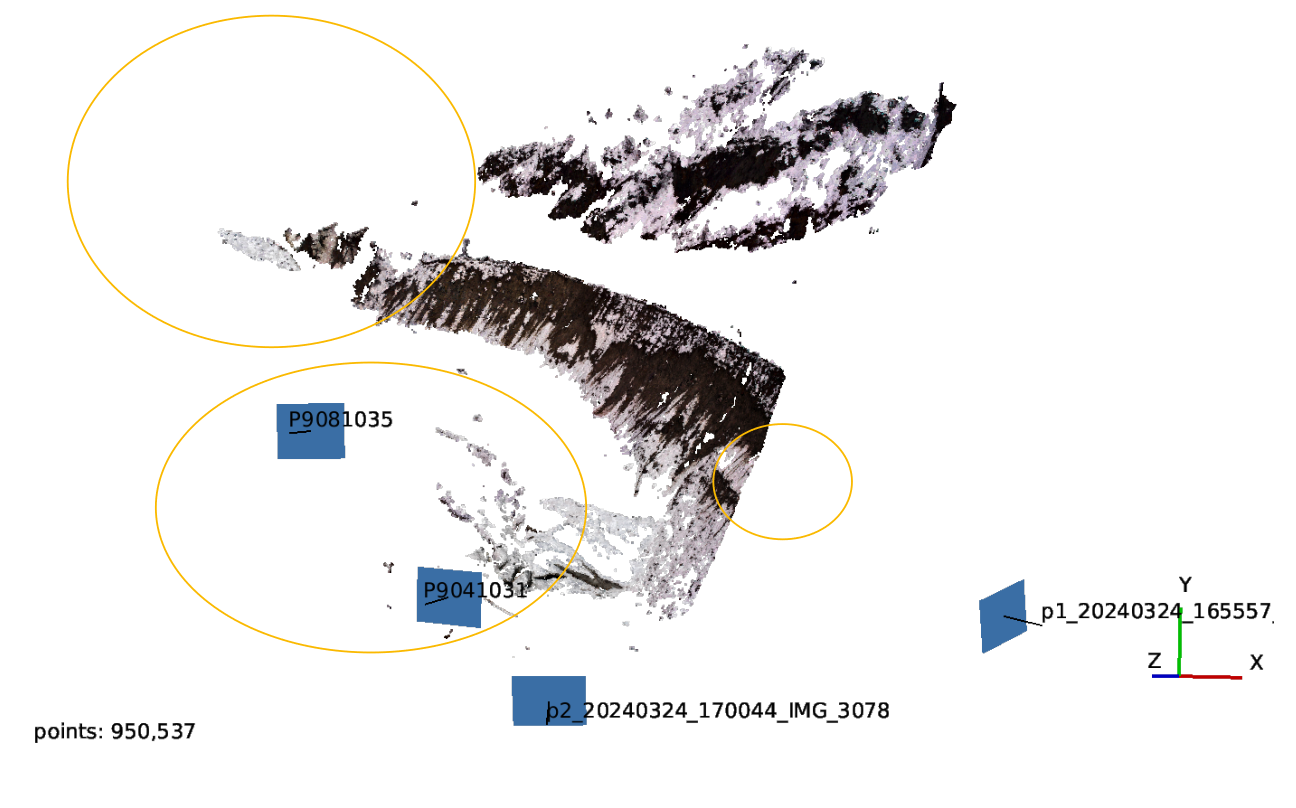
\includegraphics[height=0.4\textheight]{winter_dense_ms}
  }
  \subcaptionbox{\label{fig:5:winter_res:roma}}{
    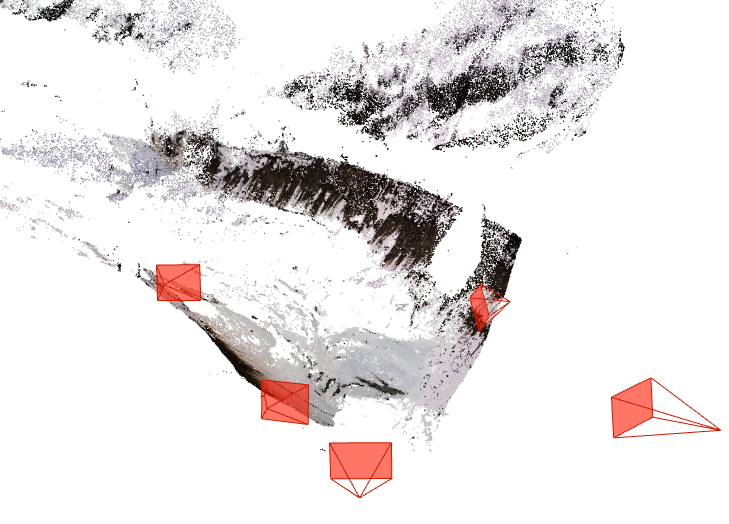
\includegraphics[height=0.4\textheight]{winter_dense_roma}
  }  
  \caption{Dense reconstruction of the Belvedere Glacier north-west lobe using (a) Agisto Metashape and (b) RoMa. The reconstruction obtained with RoMa was computed starting from the camera poses estimated with SuperPoint+LightGlue.}
  \label{fig:5:winter_res}
\end{figure}

DIM was also used to generate a dense reconstruction of the scene using the RoMa semi-dense matching algorithm for pixel-wise correspondence estimation. 
Since RoMa is a detector-free approach, correspondences are limited to image pairs. 
Therefore RoMa-derived corresponding points could not be reliably tracked across multiple images. 
While this is not ideal for image orientation, it is suitable for dense reconstruction, providing that a good geometric verification of the correspondence and some cleaning is carried out.
Because of this reason, RoMa correspondences were triangulated using the camera poses estimated within the SuperPoint+SuperGlue solution.
Similar to the orientation procedure, a brute-force matching strategy was applied, with images being matched at full resolution using a tiling approach.

\figref{fig:5:winter_res:roma} shows the resulting semi-dense reconstruction using RoMa. 
This DIM-generated reconstruction was then compared to the one generated by Agisoft Metashape using its proprietary algorithm (\figref{fig:5:winter_res:ms}).

........


\subsection{Historical internet images}

\begin{table}[ht]
    \centering
    \caption{Summary of the Nadar dataset results obtained with DIM compared to those obtained with COLMAP (with RootSIFT features) and Agisoft Metashape with its proprietary feature extractor and matches. (*) The dataset has been oriented by combining different local features: SIFT, KeyNey + HardNet, ALIKED, SuperPoint, and DISK.} 
    \label{tab:5:statistics_summary}
    
    \begin{tabular}{l p{3.5cm} p{2.2cm} p{2.2cm} p{2.2cm} p{2.2cm}}
    \toprule
    &Local features \newline and matcher & Oriented/ \newline total images & Mean reprojection error \newline [px] & Mean track \newline length &  3D tie points\\
    \midrule
    B1 &DIM \newline (combination of LF)\textsuperscript{*}    & \textcolor{green}{12/12}     & 1.09  & 2.6   & 2791 \\
    B2 &COLMAP \newline(RootSIFT)                     & 0/12      & NA    & NA    & NA   \\
    B3 &Metashape \newline (proprietary)              & 03/12     & 0.36  & 2.0   & 294  \\
    \bottomrule
    \end{tabular}
\end{table}

Dataset B – Nadar – is a collection of 12 self-portrait images from the opera Revolving (1865) of Gaspard-Félix Tournachon, known as Nadar\footnote{Wikipedia Nadar page: \url{https://en.wikipedia.org/wiki/Nadar}}. 
The images have been downloaded from Wikipedia (resolution of 524 x 671 px), and they show significantly different viewpoints, low radiometric quality, and many time-related artifacts. 
In addition, the dataset is partially ill-posed for photogrammetric purposes since Nadar sometimes changed both facial expressions and the relative position between the head and shoulders. 
All these characteristics make the reconstruction difficult with classical approaches.

\begin{figure}
    \centering
    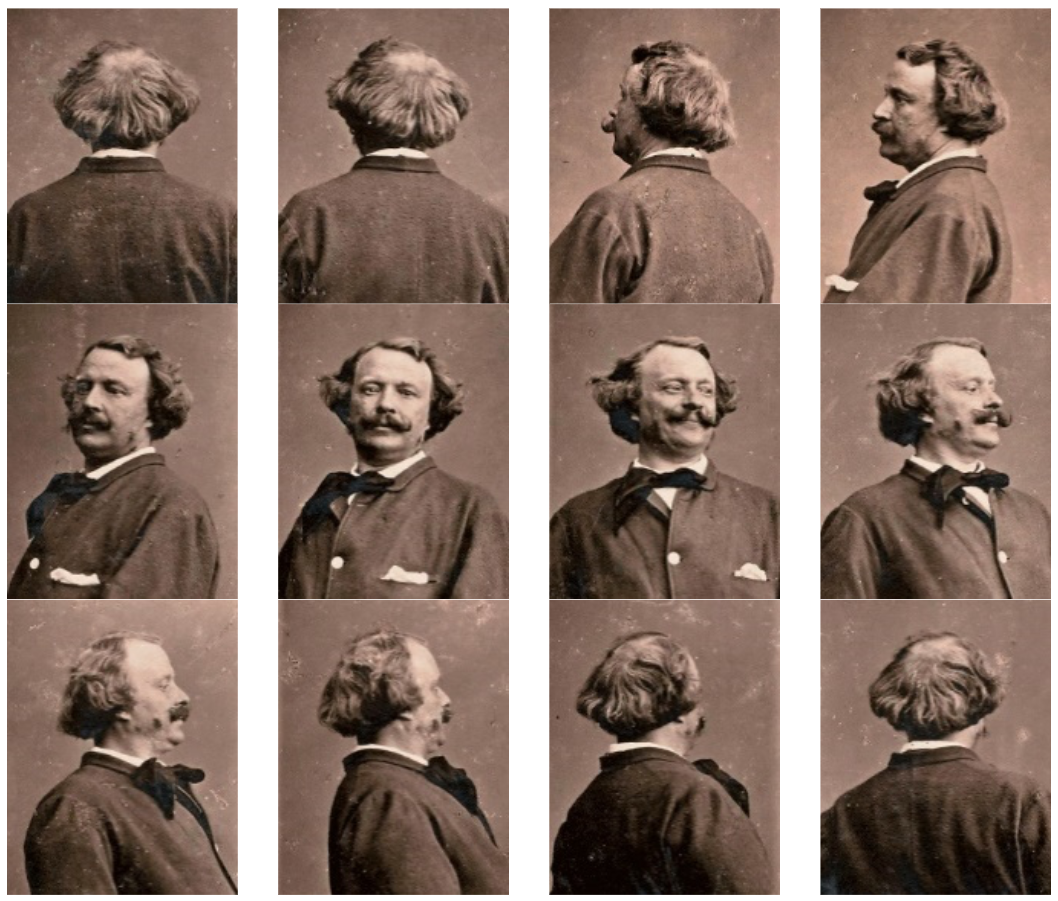
\includegraphics[width=0.6\textwidth]{nadar_images}
    \caption{Sample images Dataset B - Nadar}
    \label{fig:5:nadar_images}
\end{figure}

For the Nadar dataset, different local features have been tested: SIFT, KeyNey + HardNet, ALIKED, SuperPoint, and DISK.
SuperPoint and DISK local features were matched with LightGlue, while the others were matched with a nearest-neighbor approach. 
None of these approaches managed to orient more than three images, except DISK which found significantly more tie points and oriented seven images. 
In \figref{fig:5:res_nadar}, a matching pair example is reported for SIFT (a) and DISK (b).
Metashape completely failed to orient the dataset. 

Only by combining all the tie points from the previous approaches, excluding Metashape, was it possible to orient the whole dataset (\figref{fig:5:res_nadar}c-d). 
Tie points with multiplicity equal to two were excluded because they were considered not sufficiently robust and prone to outliers. 
In addition, no ratio threshold has been used to retain more matches. 
Because of the camera network and the scarcity of tie points, images were first oriented using a rough nominal focal length, then focal length and one radial distortion parameter were updated in a final bundle adjustment with self-calibration.

Concerning 3D model reconstruction, the poor radiometry of the images caused the dense matching of COLMAP and Metashape to fail. 
Therefore, to obtain a point cloud dense enough to build a meshed textured 3D model, the deep learning-based semi-dense matcher RoMA available in DIM is applied (\figref{fig:5:res_nadar}e-f). 
Finally, using Metashape functionalities, a textureized model is created (\figref{fig:5:res_nadar}g-h).

\begin{figure}
  \centering
  \subcaptionbox{SIFT\label{fig:5:res_nadar:1}}{
    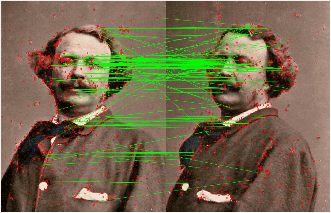
\includegraphics[height=2.3cm]{res_nadar_1.png}
  }
  \subcaptionbox{DISK\label{fig:5:res_nadar:2}}{
    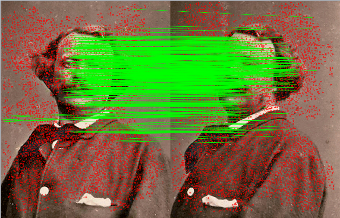
\includegraphics[height=2.3cm]{res_nadar_2.png}
  }
  \subcaptionbox{camera poses\label{fig:5:res_nadar:3}}{
    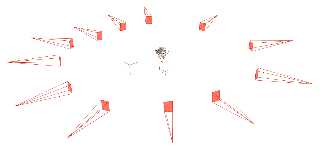
\includegraphics[height=2.3cm]{res_nadar_3.png}
  }
  \subcaptionbox{3D tie points - close up\label{fig:5:res_nadar:4}}{
    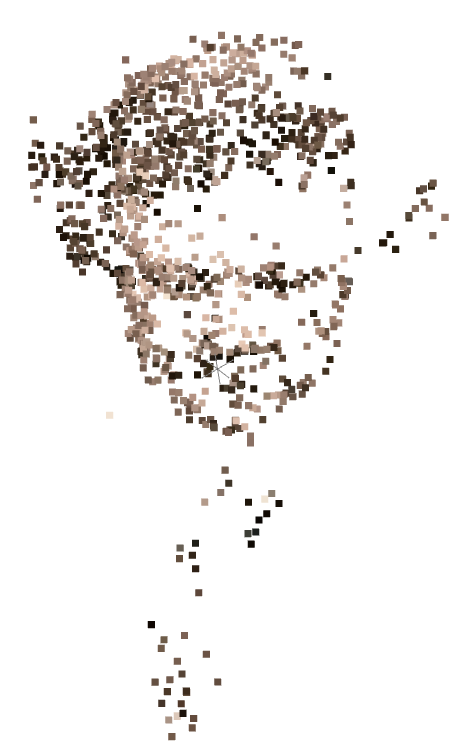
\includegraphics[height=2.3cm]{res_nadar_4.png}
  } \\
  \subcaptionbox{dense cloud - front\label{fig:5:res_nadar:5}}{
    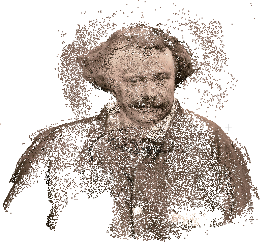
\includegraphics[height=2.3cm]{res_nadar_5.png}
  } \qquad
  \subcaptionbox{dense cloud - back\label{fig:5:res_nadar:6}}{
    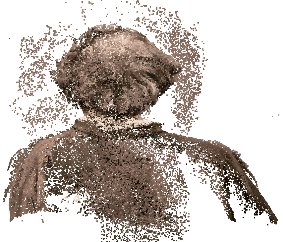
\includegraphics[height=2.3cm]{res_nadar_6.png}
  } \qquad
  \subcaptionbox{mesh with texture~--~front\label{fig:5:res_nadar:7}}{
    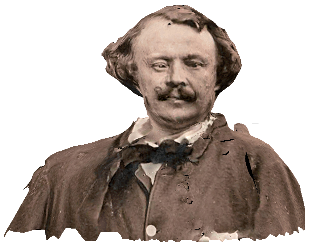
\includegraphics[height=2.3cm]{res_nadar_7.png}
  } \qquad
  \subcaptionbox{mesh with texture - back\label{fig:5:res_nadar:8}}{
    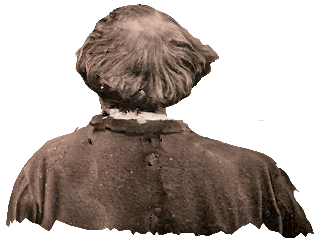
\includegraphics[height=2.3cm]{res_nadar_8.png}
  }
  \caption{Results for Nadar dataset. (a) SIFT matches and (b) DISK matches on an image pair; (c) camera poses and (d) 3D tie points; (e-f) semi-dense point cloud generated from RoMA tie points; (g-h) textured mesh 3D model.}
  \label{fig:5:res_nadar}
\end{figure}

\subsection{Combining UAV and terrestrial images}

\begin{figure}
  \centering
    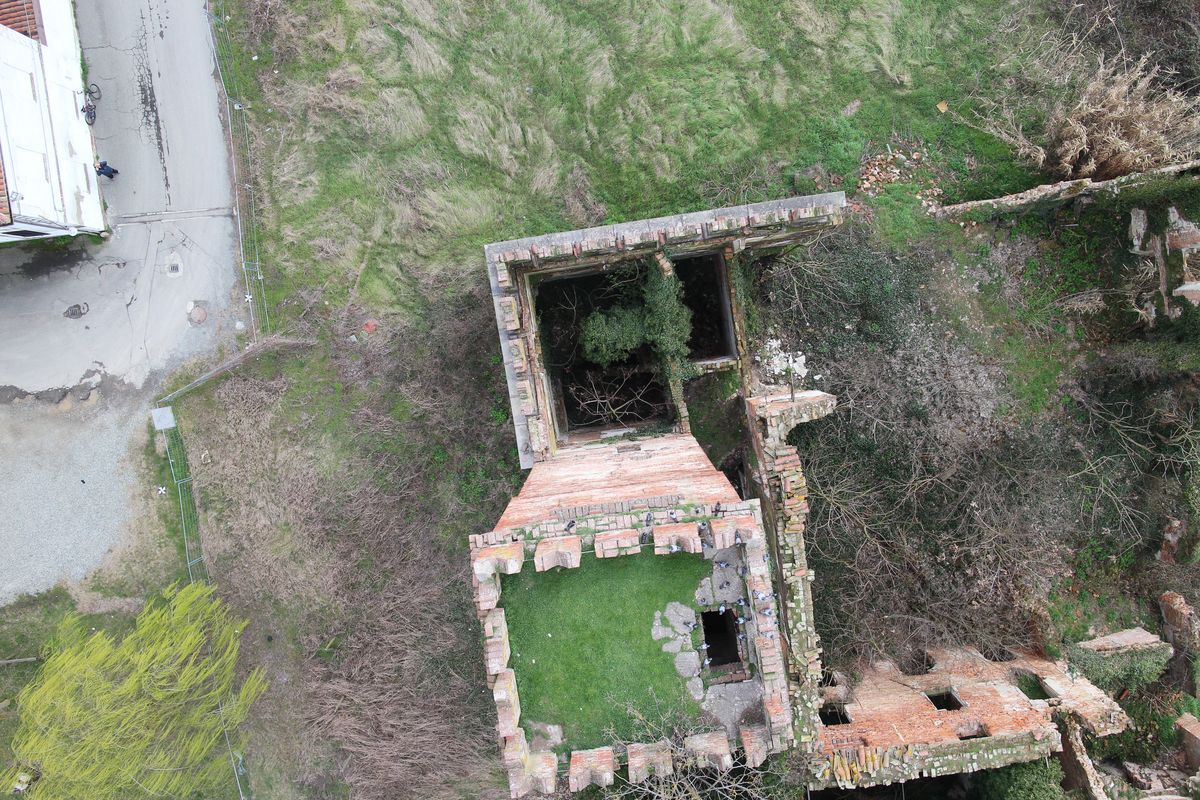
\includegraphics[height=3cm]{castle_img_1}
    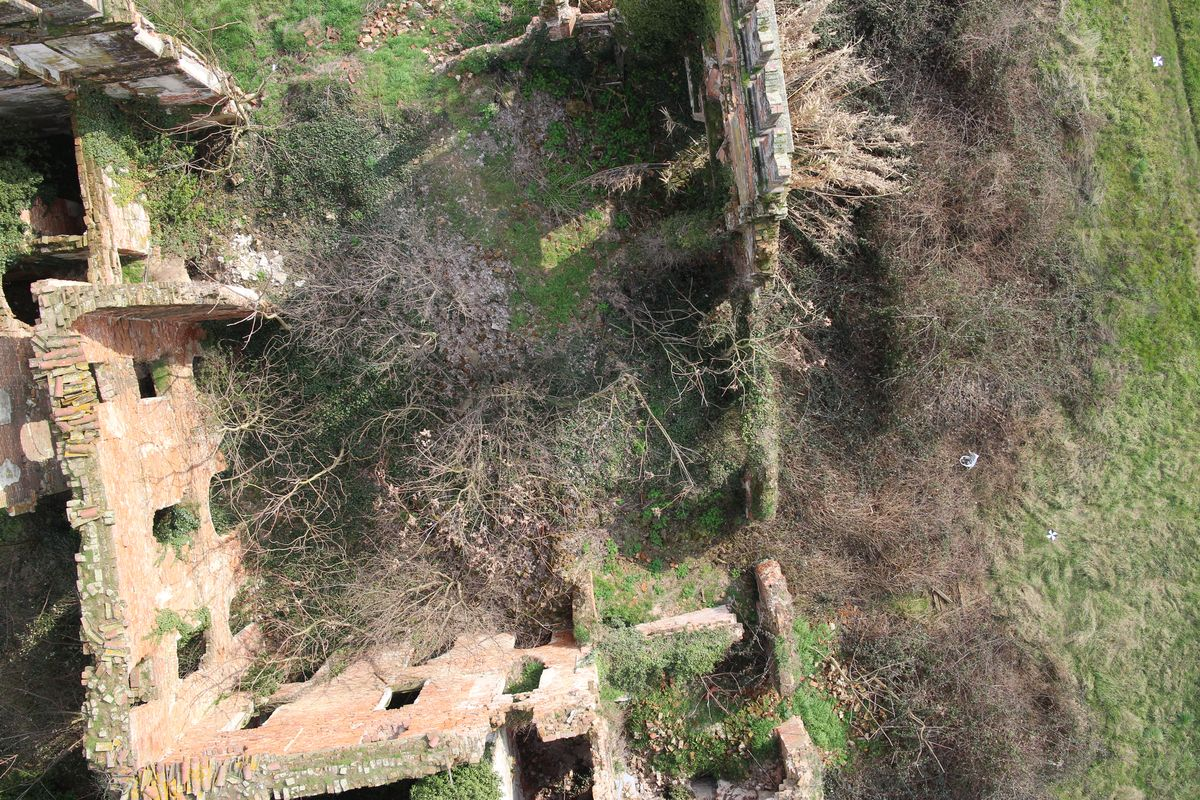
\includegraphics[height=3cm]{castle_img_2}
    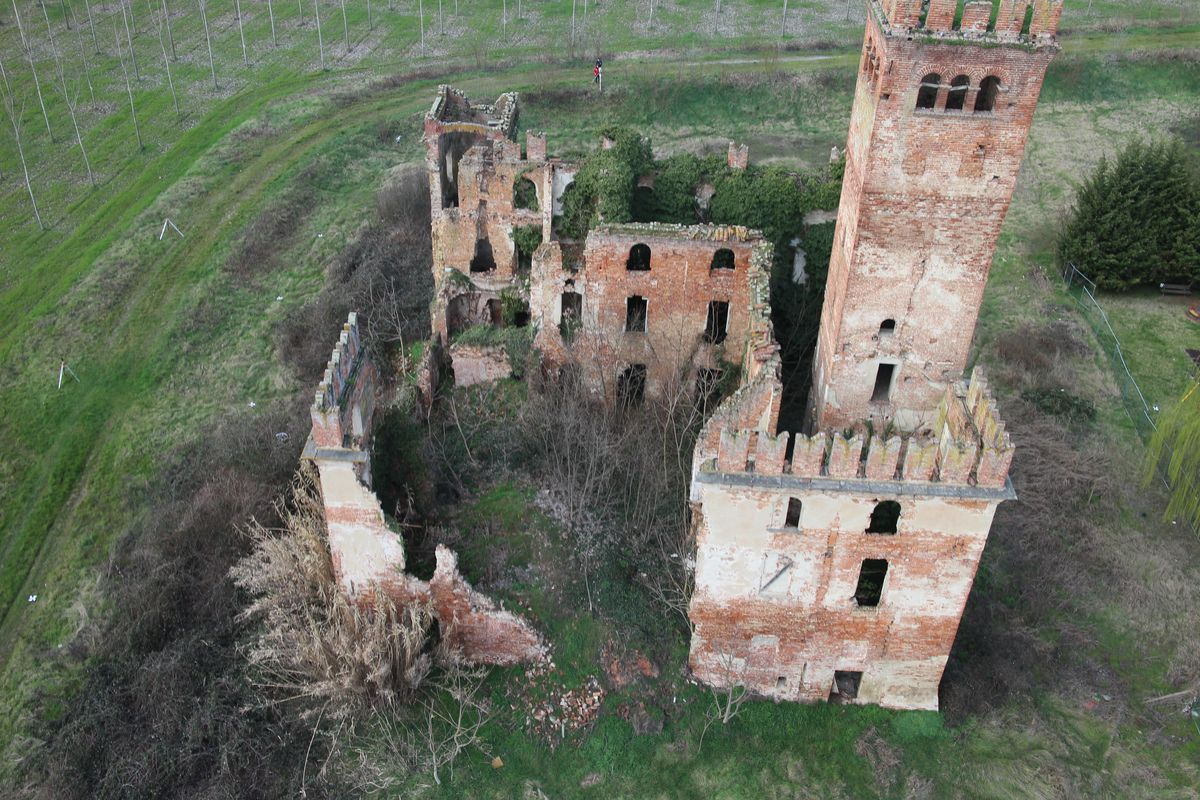
\includegraphics[height=3cm]{castle_img_3} \\
    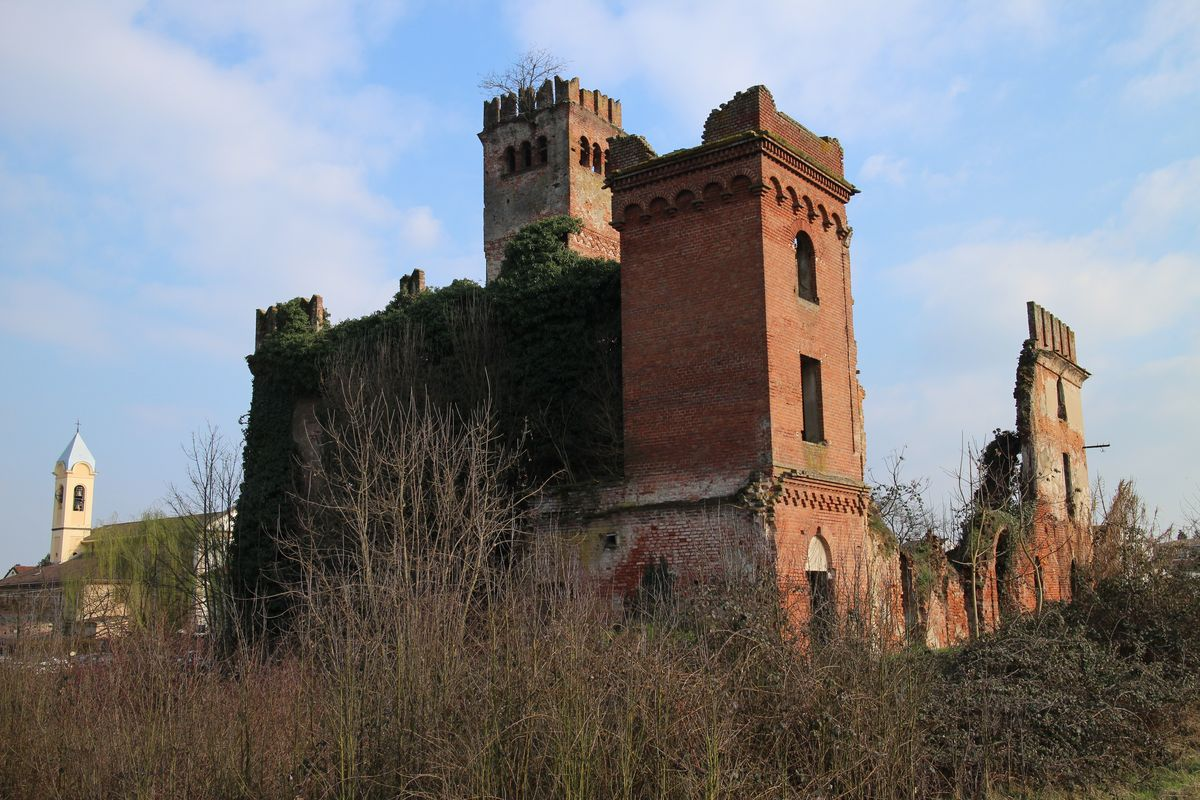
\includegraphics[height=3cm]{castle_img_4}
    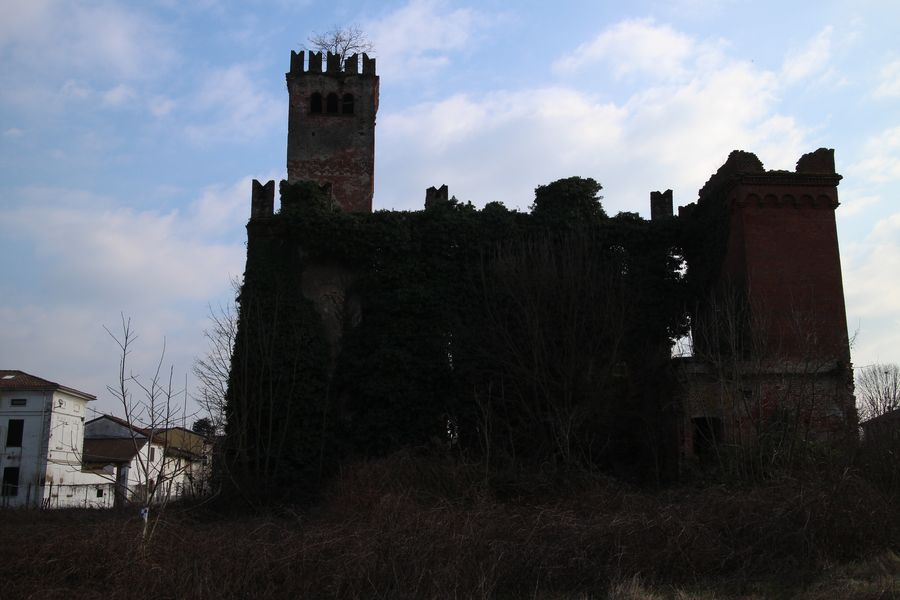
\includegraphics[height=3cm]{castle_img_5}
    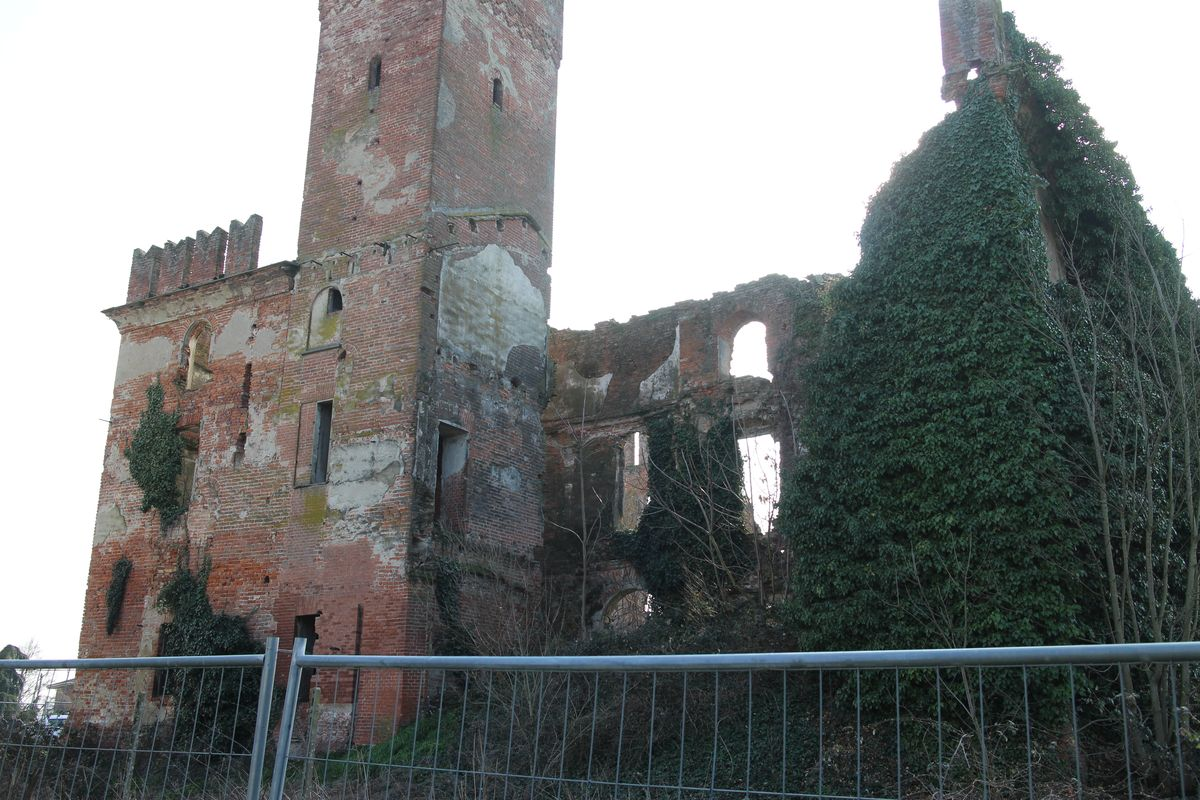
\includegraphics[height=3cm]{castle_img_6}
  \caption{Sample images Dataset C - Castle. Images in the first row are samples of the nadiral and oblique UAV images, those in the second row are samples of the terrestrial images, including some of the challenging underexposed or overexposed images.}
  \label{fig:5:castle_img}
\end{figure}

\begin{figure}
  \centering
    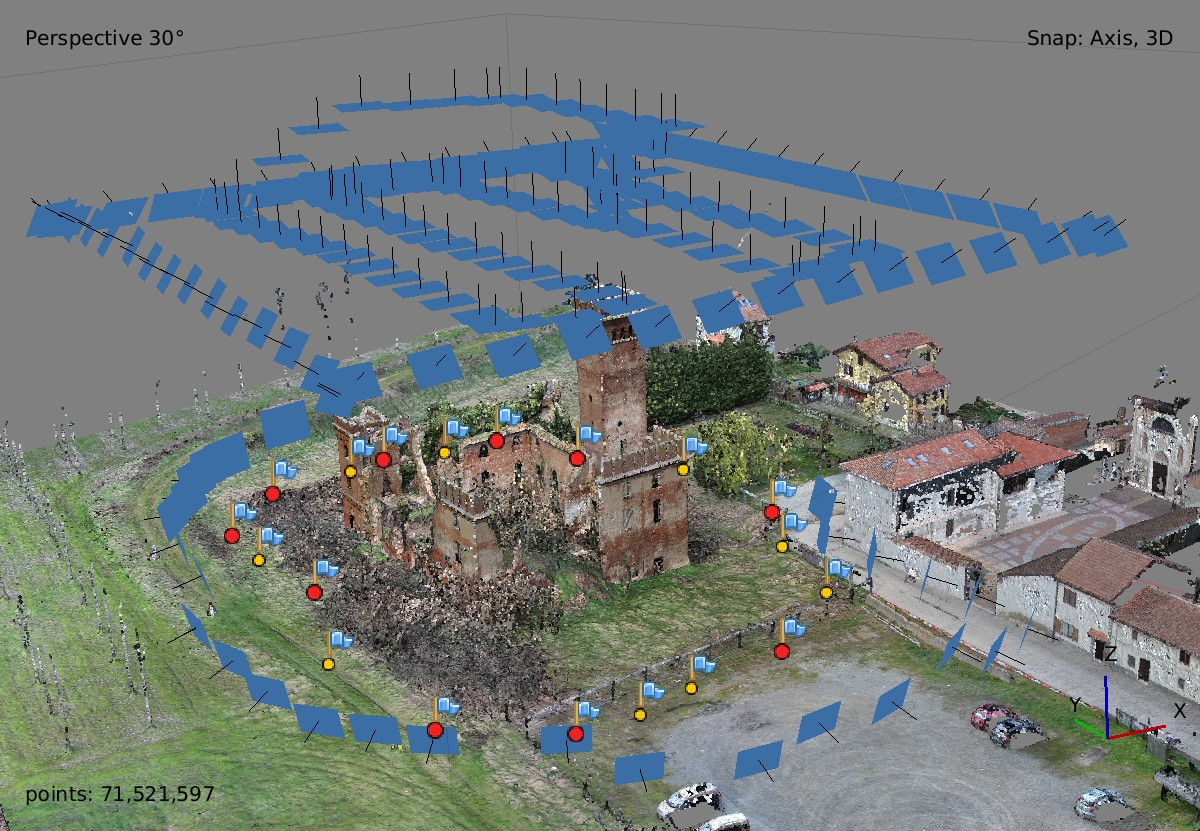
\includegraphics[width=0.6\textwidth]{castle_gt}
  \caption{Dataset C\_GT, used as the ground truth to evaluate the results on Dataset C. The red flags are the targets used as GCPs while the yellow ones those used as CPs.}
  \label{fig:5:castle_gt}
\end{figure}


\begin{table}[ht]
    \centering
    \caption{Summary of the Castle dataset results obtained with DIM, compared to the results obtained with COLMAP (with RootSIFT features) and Agisoft Metashape with its proprietary feature extractor and matches. (*) As COLMAP produced two non-linked reconstructions, the reported results refer to the reconstruction with the highest number of oriented images.} 
    \label{tab:5:castle_statistics}
    
    \begin{tabular}{l p{3.5cm} p{2.2cm} p{2.2cm} p{2.2cm} p{2.2cm}}
    \toprule
    & Local features \newline and matcher & Oriented/ \newline total images & Mean reprojection error \newline [px] & Mean track \newline length &  3D tie points\\
    \midrule
    C1 &DIM: SuperPoint \newline + LightGlue           & \textcolor{green}{48/48}     & 0.9   & 3.3   & 75274 \\
    C2 &COLMAP \newline (RootSIFT)\textsuperscript{*} & 31/48     & 0.94  & 3.7   & 11367 \\
    C3 &Metashape \newline (proprietary)               & \textcolor{green}{48/48}     & 0.5   & 2.5   & 59679 \\ 
    \bottomrule
    \end{tabular}
\end{table}


Dataset C – Castle – is composed of 48 images of the half-destroyed historical Castle of Casalbagliano, Alessandria (Italy). 
It is a traditional photogrammetric dataset of a cultural heritage site including 25 nadiral UAV images, 11 oblique UAV images, and 12 terrestrial images \figref{fig:5:castle_img}, with a camera network like a classical photogrammetric survey. 
Dataset C is the only one with an available ground truth. 
All the images of Dataset C were acquired by a single Canon Eos M with a fixed focal length of 22 mm and a size of 5184 x 3456 px.
The UAV nadiral images exhibit a modest overlap, approximately 60\% in the longitudinal direction and 40\% in the transversal direction. 
The UAV oblique images consist of four convergent shots acquired at each corner of the block, along with five additional images positioned along the exterior perimeter. 
The terrestrial images are acquired along a circle all around the castle. 
The main challenge of this dataset is linking together the nadiral UAV images with the terrestrial ones, as they have a strongly different point of view. 
Moreover, some of the terrestrial images are underexposed and characterized by large dark areas or acquired against the sun and therefore they show strong sunlight reflections. 

Dataset C was extracted from a larger and more robust dataset, named Dataset C\_GT \figref{fig:5:castle_gt}, and which was used as a ground truth reference to validate the results obtained with DIM.
This dataset is composed of 172 images (83 nadiral, 61 oblique, and 28 terrestrial) with an average overlap between the images between 70\% and 80\% and an average GSD of approximately 9 mm \cite{Gagliolo2017_uav_conservation_histo, gagliolo2018_parameter_optim}. 
The full dataset also included 19 targets deployed on the ground around the castle and measured by a total station with sub-centimetric accuracy. Dataset C\_GT was processed with Metashape, by using 10 targets as GCPs and performing a self-calibration of the camera. The quality of the photogrammetric block was evaluated on the remaining 9 targets, used as CPs, resulting in an overall RMSE of 1.9 cm in the three directions.

\begin{figure}
    \centering
    % \begin{tabular}{cc} % Create the 2x2 grid
    %     \begin{tabular}{c} % First column, top cell
    %         \subcaptionbox{SuperPoint+LightGlue\label{fig:5:castle:dim}}{
    %             \includegraphics[height=3cm]{castle_matches_splg}
    %         } \\ % End of first cell
    %         \subcaptionbox{COLMAP RootSIFT\label{fig:5:castle:colmap}}{
    %             \includegraphics[height=3cm]{castle_matches_colmap}
    %         } 
    %     \end{tabular} & % Start the second column
    %     \subcaptionbox{Agisoft Metashape\label{fig:5:castle:metashape}}{
    %         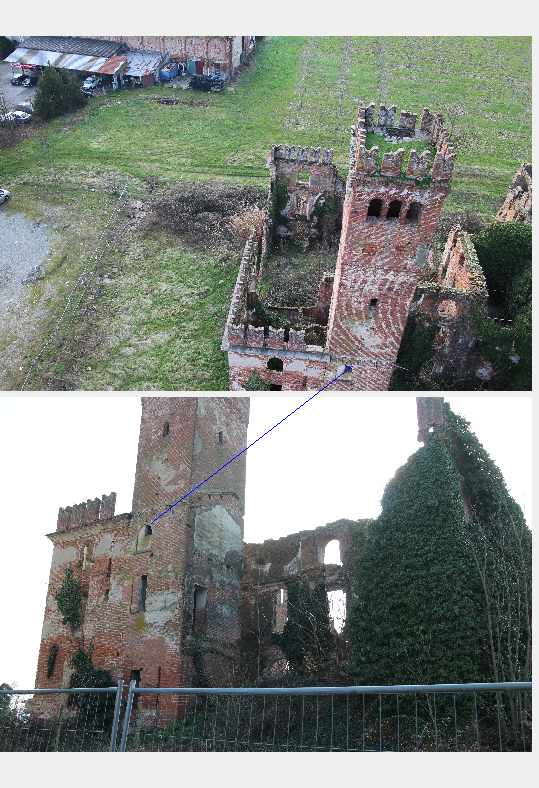
\includegraphics[height=5cm]{castle_matches_ms}
    %     } 
    % \end{tabular}
    \subcaptionbox{SuperPoint+LightGlue\label{fig:5:castle:dim}}{
        \includegraphics[height=4cm]{castle_matches_splg}
    } \\ 
    \subcaptionbox{COLMAP RootSIFT\label{fig:5:castle:colmap}}{
        \includegraphics[height=4cm]{castle_matches_colmap}
    } \\
    \subcaptionbox{Agisoft Metashape\label{fig:5:castle:metashape}}{
        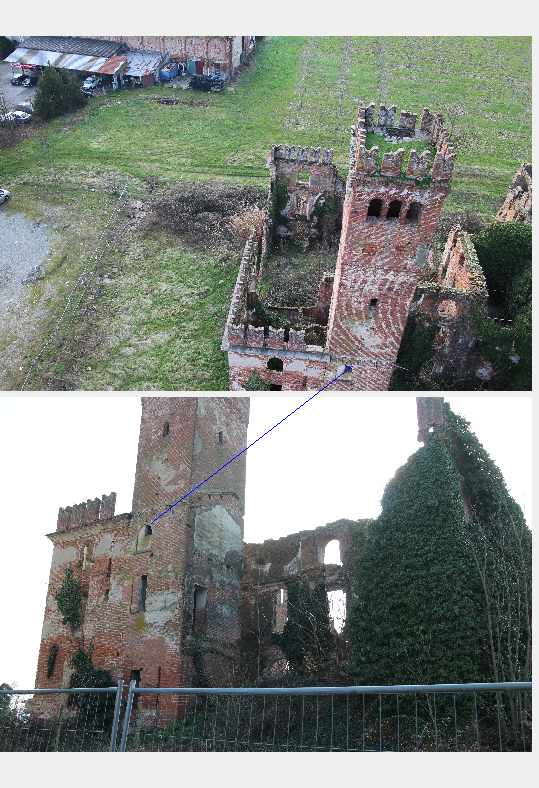
\includegraphics[height=8.5cm]{castle_matches_ms}
    } 
    \caption{Example of matched features with the different approaches on a challenging image pair (green or blue lines are the valid matches, while the red dots are the rejected keypoints): (a) SuperPoint + LightGlue (658 valid matches); (b) COLMAP RootSIFT (49 valid matches); (c) Agisoft Metashape (1 valid match).}
    \label{fig:5:castle_matches}
\end{figure}

\begin{figure}
  \centering
  \subcaptionbox{\label{fig:5:castle_rec:splg}}{
    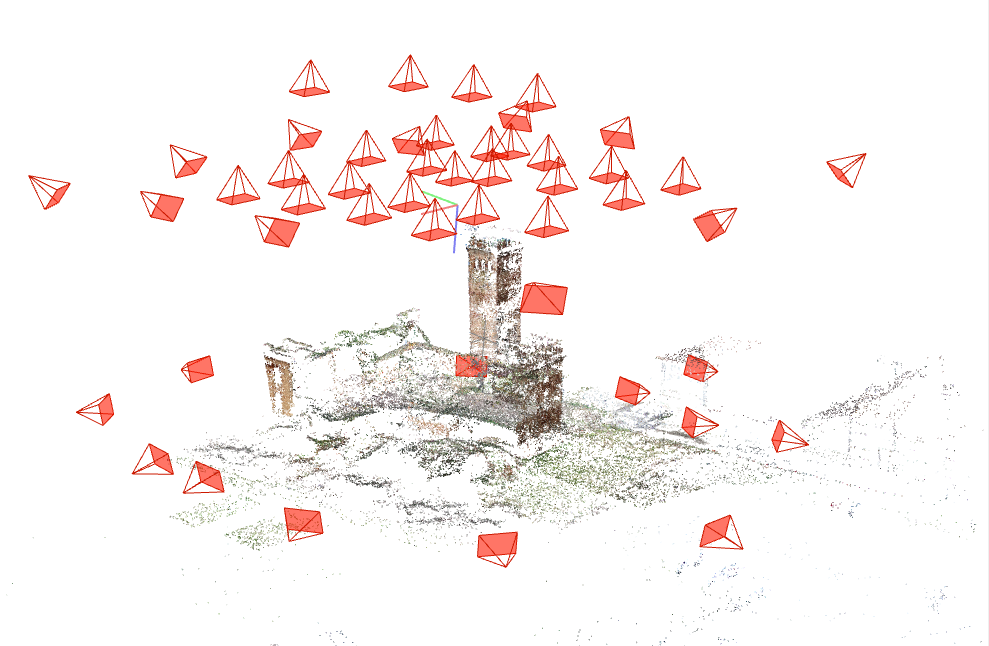
\includegraphics[height=4.5cm]{castle_rec_splg.png}
  }
  \subcaptionbox{\label{fig:5:castle_rec:georef}}{
    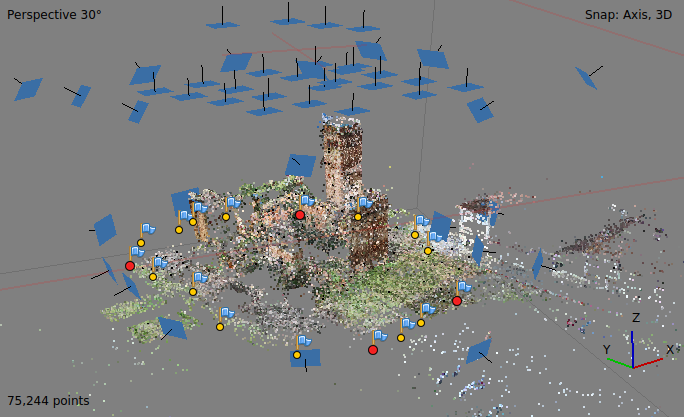
\includegraphics[height=4.5cm]{castle_rec_splg_georef.png}
  }
  \caption{(a) Reconstructed sparse point cloud and oriented camera with SuperPoint + LightGlue after the bundle in COLMAP; (b) the same solution from Metashape, georeferenced with 4 GCPs (red flags), while all the other points are used as CPs (yellow flags)}
  \label{fig:5:castle_rec}
\end{figure}

Similar to Dataset A, Dataset C was processed with DIM by using the SuperPoint+LightGlue pipeline. 
However, due to the larger number of images, a low-resolution guided approach was used for image pair selection to reduce computational time. 
Images were first downsampled and matched using a fast brute-force method. 
All pairs with at least 30 valid matches were then selected for the full-resolution matching stage.  
As before, images were first upscaled by a factor of two with a bicubic interpolation prior to feature extraction, which was again performed using a tile-based approach.

The results obtained with SuperPoint + LightGlue (\tabref{tab:5:statistics_summary}) were significantly better only compared to those obtained with a traditional COLMAP processing pipeline (C2), while they were similar to the outcomes obtained with Metashape (C3). 
With both LightGlue and Metashape, all 48 images were oriented. On the other hand, COLMAP failed to orient all the images together, but it created two different not-linked models. The largest model consisted of only 31 oriented images, as detailed in \tabref{tab:5:statistics_summary}. 
The smallest average reprojection error of 0.5 px was obtained by processing the dataset using Metashape with its proprietary local feature implementation, while a slightly higher reprojection error of 0.9 px was obtained by SuperPoint + LightGlue (\tabref{tab:5:statistics_summary}), as SuperPoint did not have subpixel accuracy in keypoint detection. 
On the other hand, the mean track length of 3.3 obtained with SuperPoint + LightGlue was larger than the 2.5 obtained with Metashape, guaranteeing higher redundancy of the observations in the bundle adjustment. 

\figref{fig:5:castle_matches} shows the matched keypoints for a challenging pair composed of a UAV oblique image and a terrestrial image, with a wide baseline and rather bad lighting conditions for the terrestrial image. 
The combination of SuperPoint + LightGlue, which works better under strong viewpoints conditions \citep{ioli2024deep}, allowed for extracting more than 600 valid matches, while Metashape was able to find only a single valid match. Surprisingly for this pair, COLMAP with RootSIFT was able to detect more matches than Metashape, probably thanks to its ability to estimate affine descriptors \cite{Lindeberg1997_affine}. 
However, for other challenging pairs, the results of SuperPoint + LightGlue were comparable to those of Metashape or COLMAP, without providing any relevant improvement. The matches obtained with SuperPoint + LightGlue were finally imported into COLMAP for the bundle adjustment and reconstruction (\figref{fig:5:castle_rec:splg}).
The two complete solutions C1 (SuperPoint + LightGlue) and C3 (pure Metashape), in which all the 48 images were oriented, were validated by importing the estimated reconstructions into a new Metashape project and adding 4 GCPs at the block corner as a minimum constraint, while leaving the other 15 targets as CPs (\figref{fig:5:castle_rec:georef}). 
This made it possible to compare the solutions C1 and C3 with the ground truth Dataset C\_GT and to evaluate the on-ground reconstruction accuracy based on the CPs and the camera pose error by comparing the camera exterior orientation parameters.
Comparable results were obtained for both C1 and C3, with a centimetric error on the CP and an average error of less than 5 cm on the camera location (\tabref{tab:5:castle_eo_stats}). 
This highlights that Dataset C was correctly oriented using both SuperPoint + LightGlue and Metashape processing, without showing a clear superiority of any approach. 

\begin{table}[ht]
    \centering
    \caption{Summary of accuracy evaluation for the solutions obtained with SuperPoint + LightGlue (C1) and Metashape (C3) with respect to the ground truth (C\_GT). The RMSE on the CPs was computed as the RMS of the difference between the 3D coordinates of the targets measured on the field and those estimated in C1 and C3. The RMSE on the cameras was computed as the RMS of the differences between the estimated 3D coordinates and attitude angles of the cameras in C\_GT and those estimated in C1 and C3.} 
    \label{tab:5:castle_eo_stats}

    \begin{tabular}{l p{2cm} p{3.5cm} p{3.5cm} p{3.5cm}} 
    \toprule
    & Approach & RMSE X/Y/Z \newline on CPs [m] & RMSE X/Y/Z \newline on camera location [m] & RMSE Yaw/Pitch/Roll \newline on camera attitude [º] \\ 
     \midrule
    C1 & SuperPoint + LightGlue & 0.017/0.010/0.010 & 0.036/0.043/0.044 & 0.13/0.04/0.07 \\
    C3 & Metashape & 0.014/0.011/0.012 & 0.043/0.040/0.041 & 0.08/0.11/0.11 \\   
    \bottomrule
    \end{tabular}
\end{table}


% \subsection{Thermal vs RGB}

% The inherent low spatial resolution and low contrast of infrared images has made the application of multi-modal image matching a significant challenge within computer vision. Whilst the most popular traditional matching approaches present suitable methods for the orientation of multiple infrared images \cite{Firmenich2011_Multispectral, Aguilera2021_multispectral}, difficulties arise matching infrared and visible images due to the sensitivities of non-linear radiation distortion (NRD) \cite{Laguela2013_thermographic, Ham2013_thermal}.
% Furthermore, concerning the use of IR-RGB image blocks, this challenge only grows when we begin to address pose, noise, and temporality \cite{Li2020_RIFT, jin_image_2021}. 
% Specifically designed to be insensitive to NRD, RIFT (Radiation Invariant Feature Transform) \cite{Li2020_RIFT} provides a SIFT-like multi-modal image matching method using frequency-domain information such as phase congruency and maximum index mapping to determine and match keypoints. 
% RIFT has established itself as the most suitable handcrafted feature-based thermal image matching method for determining correspondences between infrared and visible imagery.
 
% However, the development of learning-based image-matching methods warrants exploration, overcoming one of the critical junctures for 3D reconstruction, image registration, and localization using thermal data \cite{velesaca_multimodal_2024}. 
% For multi-modal image matching, the ability to overcome these challenges has justified their exploration for infrared-visible image matching. 
% \citet{RuizDeOna2023_photomatch}’s PhotoMatch multi-modal image matching software demonstrates the application of DL image matching methods, notably ‘detect-and-describe’ approaches like D2-Net \cite{Dusmanu2019_d2net} and R2D2 \cite{revaud2019r2d2}, with both approaches superior to hand-crafted methods in six multi-modal scenarios. 
% Similarly, \cite{chang_speed_2024} presents a novel lightweight network built to exploit local and global feature information for infrared-visible image matching, achieving competitive results with RIFT, R2D2, SuperPoint+LightGlue, and LoFTR.
% These cases demonstrate the benefit that can be gained from learning-based methods for thermal image matching and the need for comparison of handcrafted- and learning-based image matching methods for thermal data fusion.

% To evaluate the matching of infrared-visible imagery, Lenton Lodge, the 19th century Grade II* listed gatehouse built by Jeffry Wyatville and former entrance to Wollaton Hall, was used as a case study in Nottingham, UK. 
% The structure, largely comprising Mansfield sandstone, represents one of the finest examples of Elizabethan Revival in England and presents an extraordinary history of disrepair and restoration. 
% Before image acquisition, a ground control survey was undertaken with a Leica TS10 and custom 3D-printed survey targets constructed from selective laser sintering, aluminum, and rubber, designed to be detectable in both infrared and visible images. 
% Images were captured at a time to maximize the ‘baking’ of the building from solar radiation and to prevent the interference of shadows around the gatehouse turrets.
% Images were captured in three strips at 4m, 8m, and 12m from the facade.

% A Workswell WIRIS Pro (WWP) UAV thermal imaging system, offering a Focal Plane array (FPA) active sensor with 640x512 resolution and a temperature sensitivity \SI{0.05}{\degreeCelsius} was used, configured to work terrestrially. 
% The WWP features both a thermal sensor and visible sensor (res. 1920x1080) fixed within the same camera unit, allowing for both RGB and IR radiation to be captured of a scene at the same time. Table \ref{} summarises WWP key properties and Fig. \ref{} shows the thermal imaging system.


% References
\makechapterbibliography{}
